\section{บทที่ 6 ระบบควบคุม การสื่อสาร และการควบคุมแบบป้อนกลับ}

\titleformat{\paragraph}[block]{\normalsize\bfseries\color{mainblue}}{}{0pt}{}
\titlespacing*{\paragraph}{0pt}{0.8em}{0.25em}

\textbf{ชื่อบทภาษาอังกฤษ:} Control Systems, Communication and Feedback Control \\
\textbf{รายวิชา:} หุ่นยนต์ในระบบงานอุตสาหกรรม (Industrial Robots) \\
\textbf{รหัสวิชา:} 5574506 \\
\textbf{หน่วยกิต:} 3(1-4-4) \\

\subsection{แนวคิดสำคัญของบท}

ระบบควบคุมของหุ่นยนต์อุตสาหกรรมไม่ได้หมายถึงเพียงโปรแกรมที่สั่งให้แขนกลเคลื่อนจากจุดหนึ่งไปยังอีกจุดหนึ่ง แต่เป็นระบบหลายชั้นที่เชื่อมโยงคำสั่งการผลิต การวางแผนการเคลื่อนที่ การควบคุมตำแหน่ง ความเร็ว และแรงบิด ตลอดจนการรับข้อมูลจากเซนเซอร์และการสื่อสารกับ PLC อุปกรณ์รอบข้าง และระบบเครือข่ายในโรงงาน

หัวใจของความแม่นยำคือ \textbf{การควบคุมแบบป้อนกลับ (Feedback Control)} ซึ่งวัดผลลัพธ์จริงแล้วเปรียบเทียบกับค่าที่ต้องการ ความคลาดเคลื่อนที่เกิดขึ้นถูกนำไปสร้างคำสั่งควบคุมใหม่อย่างต่อเนื่อง จึงช่วยลดผลกระทบจากการเปลี่ยนแปลงของโหลด แรงเสียดทาน ความคลาดเคลื่อนของพารามิเตอร์ และสิ่งรบกวนภายนอก อย่างไรก็ตาม การป้อนกลับที่ออกแบบไม่เหมาะสมอาจทำให้ระบบสั่น เกิด Overshoot หรือสูญเสียเสถียรภาพได้

ในระบบหุ่นยนต์จริง การควบคุมระดับข้อต่อมักใช้โครงสร้างวงรอบซ้อน (Cascade Control) ได้แก่ วงรอบกระแสหรือแรงบิดที่อยู่ด้านใน วงรอบความเร็ว และวงรอบตำแหน่งที่อยู่ด้านนอก ขณะที่ Robot Controller รับคำสั่งระดับสูง เช่น จุดปลายทาง ท่าทาง ความเร็ว และเงื่อนไขลำดับงาน แล้วแปลงเป็นค่าคำสั่งให้แต่ละแกน

การบูรณาการหุ่นยนต์เข้ากับสายการผลิตต้องอาศัยการสื่อสารหลายระดับ ตั้งแต่สัญญาณ Digital I/O แบบเดินสายตรง ไปจนถึง Fieldbus, Industrial Ethernet, OPC UA และซอฟต์แวร์เชื่อมต่อระดับระบบ การเลือกวิธีสื่อสารต้องพิจารณาทั้งความเร็ว ความเป็น Deterministic ปริมาณข้อมูล ความสามารถในการวินิจฉัย ความเข้ากันได้ ความปลอดภัย และต้นทุนตลอดอายุระบบ

\begin{quote}
\textbf{สาระสำคัญ:} ความแม่นยำของหุ่นยนต์เกิดจากการทำงานร่วมกันของแบบจำลอง ตัวควบคุม เซนเซอร์ แอคชูเอเตอร์ เครือข่ายสื่อสาร และตรรกะลำดับงาน ไม่ได้เกิดจากอุปกรณ์ใดอุปกรณ์หนึ่งเพียงลำพัง
\end{quote}

\subsection{ความรู้พื้นฐานก่อนเรียน}

ก่อนเรียนบทนี้ ผู้เรียนควรมีพื้นฐานดังต่อไปนี้

\begin{enumerate}
    \item โครงสร้างพื้นฐานของหุ่นยนต์อุตสาหกรรม ข้อต่อ แกน และ End Effector
    \item หลักการทำงานของ Servo Motor, Servo Drive และ Encoder
    \item สัญญาณไฟฟ้าพื้นฐาน ได้แก่ Digital Input/Output, Analog Voltage และ Analog Current
    \item แนวคิดพื้นฐานของ PLC และ Ladder Diagram
    \item สมการเชิงอนุพันธ์ ฟังก์ชันถ่ายโอน และการแปลงลาปลาซในระดับเบื้องต้น
    \item แนวคิดเรื่องตำแหน่ง ความเร็ว ความเร่ง แรง และแรงบิด
    \item ความปลอดภัยในห้องปฏิบัติการไฟฟ้าและระบบอัตโนมัติ
\end{enumerate}

หากผู้เรียนยังไม่มีพื้นฐานด้านฟังก์ชันถ่ายโอน ผู้สอนสามารถเริ่มจาก Block Diagram และความสัมพันธ์เชิงเหตุผลก่อน แล้วจึงเชื่อมโยงเข้าสู่สมการเมื่อจำเป็น

\newpage

\subsection{คำสำคัญประจำบท}

\begin{table}[htbp]
    \centering
    \small
    \begin{tabularx}{\textwidth}{@{}L{0.23\textwidth} L{0.24\textwidth} X@{}}
        \hline
        \textbf{คำศัพท์ภาษาไทย} & \textbf{ภาษาอังกฤษ} & \textbf{ความหมายโดยย่อ} \\
        \hline
        ระบบควบคุมวงเปิด & Open-loop control & ระบบที่ไม่มีการวัดผลลัพธ์ย้อนกลับเพื่อแก้ไขคำสั่ง \\
        ระบบควบคุมวงปิด & Closed-loop control & ระบบที่ใช้ค่าป้อนกลับเปรียบเทียบกับค่าตั้ง \\
        ค่าตั้ง & Setpoint / Reference & ค่าที่ต้องการให้ระบบติดตาม \\
        ความคลาดเคลื่อน & Error & ผลต่างระหว่างค่าตั้งกับค่าที่วัดได้ \\
        สิ่งรบกวน & Disturbance & ปัจจัยภายนอกที่ทำให้ผลลัพธ์เบี่ยงเบน \\
        ตัวควบคุม PID & PID Controller & ตัวควบคุมที่รวมผลแบบสัดส่วน ปริพันธ์ และอนุพันธ์ \\
        เวลาขาขึ้น & Rise Time & เวลาที่ผลตอบสนองเพิ่มจากช่วงต่ำไปยังช่วงใกล้ค่าปลายทาง \\
        ค่าพุ่งเกิน & Overshoot & ค่าสูงสุดที่เกินค่าปลายทาง \\
        เวลาคงตัว & Settling Time & เวลาที่ผลตอบสนองเข้าสู่แถบความคลาดเคลื่อนที่กำหนด \\
        ความคลาดเคลื่อนคงตัว & Steady-state Error & ความคลาดเคลื่อนที่เหลือเมื่อเวลาผ่านไปมาก \\
        การควบคุมตำแหน่ง & Position Control & ควบคุมมุมข้อต่อหรือตำแหน่งให้ติดตามค่าคำสั่ง \\
        การควบคุมความเร็ว & Speed Control & ควบคุมอัตราการหมุนหรือความเร็วเชิงเส้น \\
        การควบคุมแรงบิด & Torque Control & ควบคุมแรงบิดมอเตอร์หรือแรงสัมผัสโดยอ้อม \\
        วงรอบซ้อน & Cascade Control & โครงสร้างหลายวงรอบที่วงด้านในตอบสนองเร็วกว่าวงด้านนอก \\
        พื้นที่ข้อต่อ & Joint Space & พื้นที่พิกัดที่อธิบายด้วยตัวแปรข้อต่อของหุ่นยนต์ \\
        พื้นที่คาร์ทีเซียน & Cartesian Space & พื้นที่พิกัดตำแหน่งและทิศทางของ End Effector \\
        เมทริกซ์จาโคเบียน & Jacobian Matrix & เมทริกซ์เชื่อมโยงความเร็วข้อต่อกับความเร็วของปลายแขน \\
        อินพุต/เอาต์พุตแบบไม่ต่อเนื่อง & Discrete I/O & สัญญาณสองสถานะ เช่น 0/1 หรือ OFF/ON \\
        การจับมือสัญญาณ & Handshake & ลำดับสัญญาณยืนยันระหว่างอุปกรณ์สองฝ่าย \\
        ฟิลด์บัส & Fieldbus & เครือข่ายดิจิทัลระดับอุปกรณ์ภาคสนาม \\
        อีเทอร์เน็ตอุตสาหกรรม & Industrial Ethernet & เครือข่าย Ethernet ที่เพิ่มกลไกให้เหมาะกับงานควบคุมอุตสาหกรรม \\
        รอบการสื่อสาร & Communication Cycle & ช่วงเวลาที่ข้อมูลควบคุมถูกแลกเปลี่ยนครบหนึ่งรอบ \\
        ความหน่วง & Latency & เวลาตั้งแต่ส่งข้อมูลจนข้อมูลมีผลที่ปลายทาง \\
        ความแปรปรวนของเวลา & Jitter & การเปลี่ยนแปลงของความหน่วงหรือคาบจากรอบหนึ่งไปอีกรอบหนึ่ง \\
        ข้อมูลแบบคาบ & Cyclic Data & ข้อมูลที่แลกเปลี่ยนซ้ำตามรอบเวลา เช่น I/O Process Data \\
        ข้อมูลแบบไม่เป็นคาบ & Acyclic Data & ข้อมูลที่ร้องขอเป็นครั้งคราว เช่น Parameter และ Diagnostic \\
        ความปลอดภัยเชิงหน้าที่ & Functional Safety & การลดความเสี่ยงด้วยฟังก์ชันควบคุมที่ผ่านการออกแบบและประเมินตามมาตรฐาน \\
        \hline
    \end{tabularx}
\end{table}

\subsection{ผลลัพธ์การเรียนรู้ประจำบท}

เมื่อเรียนจบบทนี้ นักศึกษาสามารถ

\begin{enumerate}
    \item \textbf{อธิบายและเปรียบเทียบ} หลักการควบคุมวงเปิดและวงปิด พร้อมยกตัวอย่างในระบบหุ่นยนต์ได้
    \item \textbf{วิเคราะห์} ส่วนประกอบของตัวควบคุม PID และผลของการปรับค่า $K_p$, $K_i$ และ $K_d$ ต่อผลตอบสนองได้
    \item \textbf{อธิบายและเลือกใช้} Position, Speed และ Torque Control รวมถึงโครงสร้างวงรอบซ้อนในระบบขับเคลื่อนหุ่นยนต์ได้
    \item \textbf{วิเคราะห์} ความแตกต่างระหว่าง Joint Space Control, Cartesian Space Control และแนวคิด Computed Torque Control ได้
    \item \textbf{ออกแบบและทดสอบ} การแลกเปลี่ยนสัญญาณระหว่าง PLC กับ Robot Controller ผ่าน Hard-wired I/O โดยใช้ Handshake และ Interlock ที่เหมาะสมได้
    \item \textbf{จำแนกและประเมิน} โปรโตคอล Fieldbus และ Industrial Ethernet ที่สำคัญ โดยพิจารณาความเร็ว ความเป็น Deterministic โทโพโลยี การวินิจฉัย และความเหมาะสมกับงานได้
\end{enumerate}

\newpage

\subsubsection{ตารางความสอดคล้องตามแนวทาง OBE}

\begin{table}[htbp]
    \centering
    \small
    \begin{tabularx}{\textwidth}{@{}L{0.09\textwidth} X X X X@{}}
        \hline
        \textbf{CLO} & \textbf{เนื้อหาที่เกี่ยวข้อง} & \textbf{กิจกรรมการเรียนรู้} & \textbf{วิธีประเมิน} & \textbf{หลักฐานการเรียนรู้} \\
        \hline
        CLO1 & วงเปิด วงปิด Block Diagram และ Disturbance & วิเคราะห์ระบบตัวอย่างและอภิปรายความเสี่ยง & คำถามทบทวนและแบบฝึกหัดพื้นฐาน & แผนภาพบล็อกและคำอธิบาย \\
        CLO2 & PID, Step Response, Gain Tuning, Anti-windup & ใบงาน 6-1 ทดลองปรับ Gain & ตารางผลทดลอง กราฟ และรายงานวิเคราะห์ & ค่า Overshoot, Settling Time และข้อสรุป \\
        CLO3 & Position, Speed, Torque และ Cascade Loop & วิเคราะห์แผนภาพ Servo Drive และกรณีเลือกโหมด & แบบฝึกหัดวิเคราะห์และการสาธิต & ตารางเปรียบเทียบโหมดควบคุม \\
        CLO4 & Joint Space, Cartesian Space, Jacobian, Computed Torque & วิเคราะห์เส้นทางและแรงบิดของหุ่นยนต์ & โจทย์คำนวณและกรณีศึกษา & สมการและเหตุผลในการเลือกวิธีควบคุม \\
        CLO5 & Digital/Analog I/O, Handshake, Interlock, Safety & ใบงาน 6-2 ต่อระบบ PLC–Robot แบบฝึก & ตรวจการต่อวงจรและ Ladder Sequence & Wiring Diagram, I/O List และผลทดสอบ \\
        CLO6 & Fieldbus, Industrial Ethernet, OSI, Topology, Diagnostics & เปรียบเทียบเครือข่ายจากข้อกำหนดงาน & รายงานสั้นและแบบฝึกหัดประยุกต์ & ตารางเลือกเครือข่ายพร้อมเหตุผล \\
        \hline
    \end{tabularx}
\end{table}

\subsection{แผนผังเนื้อหาของบท}

\begin{center}
\textbf{แนวคิดระบบควบคุมและการสื่อสารของหุ่นยนต์อุตสาหกรรม}\\
\vspace{0.2cm}
$\downarrow$ \\
\vspace{0.2cm}
\textbf{Open-loop และ Closed-loop}\\
\vspace{0.2cm}
$\downarrow$ \\
\vspace{0.2cm}
\textbf{สมรรถนะของผลตอบสนองและเสถียรภาพ}\\
\vspace{0.2cm}
$\downarrow$ \\
\vspace{0.2cm}
\textbf{PID Control และการปรับ Gain}\\
\vspace{0.2cm}
$\downarrow$ \\
\vspace{0.2cm}
\textbf{Position–Speed–Torque Cascade Control}\\
\vspace{0.2cm}
$\downarrow$ \\
\vspace{0.2cm}
\textbf{Joint Space และ Cartesian Space Control}\\
\vspace{0.2cm}
$\downarrow$ \\
\vspace{0.2cm}
\textbf{PLC–Robot I/O, Handshake และ Interlock}\\
\vspace{0.2cm}
$\downarrow$ \\
\vspace{0.2cm}
\textbf{Fieldbus และ Industrial Ethernet}\\
\vspace{0.2cm}
$\downarrow$ \\
\vspace{0.2cm}
\textbf{Topology, Cycle Time, Latency, Jitter และ Diagnostics}\\
\vspace{0.2cm}
$\downarrow$ \\
\vspace{0.2cm}
\textbf{การเลือกสถาปัตยกรรมควบคุมและสื่อสารสำหรับเซลล์หุ่นยนต์}
\end{center}

\newpage

\subsection{บทนำ}

หุ่นยนต์ในสายการผลิตต้องทำงานซ้ำเดิมด้วยความแม่นยำสูง แต่สภาพการทำงานจริงไม่คงที่ ชิ้นงานอาจมีมวลต่างกัน ตำแหน่งจับอาจคลาดเคลื่อน แรงเสียดทานเปลี่ยนตามอุณหภูมิ และแรงกระแทกจากภายนอกอาจรบกวนการเคลื่อนที่ หากระบบสั่งมอเตอร์ด้วยคำสั่งคงที่โดยไม่ตรวจสอบผลลัพธ์ ความคลาดเคลื่อนจะสะสมและอาจทำให้หุ่นยนต์หยิบชิ้นงานผิดตำแหน่งหรือชนอุปกรณ์

Servo System จึงใช้ Encoder หรือ Resolver วัดตำแหน่งและความเร็ว แล้วส่งข้อมูลกลับไปยัง Servo Drive หรือ Robot Controller ตัวควบคุมคำนวณความคลาดเคลื่อนและปรับแรงบิดมอเตอร์ให้เหมาะสม กระบวนการนี้เกิดขึ้นซ้ำด้วยคาบเวลาสั้นมากจนผู้ใช้งานมองเห็นเป็นการเคลื่อนที่ต่อเนื่อง

ในระดับเซลล์การผลิต หุ่นยนต์ต้องรอเงื่อนไขจาก PLC เช่น ประตูนิรภัยปิด ชิ้นงานพร้อม Gripper พร้อม และสถานีถัดไปว่าง เมื่อเงื่อนไขครบ PLC จึงส่งคำสั่งเริ่มโปรแกรม หุ่นยนต์ตอบกลับสถานะ Running, Complete หรือ Fault การแลกเปลี่ยนข้อมูลนี้อาจทำผ่านสาย Digital I/O หรือเครือข่ายอุตสาหกรรม

ดังนั้น การออกแบบระบบหุ่นยนต์ต้องตอบคำถามอย่างน้อยสามระดับ

\begin{enumerate}
    \item \textbf{ระดับการเคลื่อนที่:} จะทำให้แต่ละแกนติดตามตำแหน่ง ความเร็ว หรือแรงบิดได้อย่างไร
    \item \textbf{ระดับลำดับงาน:} PLC และ Robot Controller จะยืนยันสถานะและควบคุม Sequence อย่างไร
    \item \textbf{ระดับเครือข่าย:} จะเลือกโปรโตคอลและโครงสร้างเครือข่ายแบบใดให้ตอบสนองทันเวลา วินิจฉัยง่าย และปลอดภัย
\end{enumerate}



\subsection{เนื้อหาและกิจกรรมการเรียนรู้}

\subsubsection{องค์ประกอบของระบบควบคุมหุ่นยนต์}

ระบบควบคุมวงปิดทั่วไปประกอบด้วยองค์ประกอบต่อไปนี้

\begin{itemize}
    \item \textbf{Reference หรือ Setpoint:} ค่าที่ต้องการ เช่น มุมข้อต่อ $30^\circ$ หรือความเร็ว $60\ \text{rad/s}$
    \item \textbf{Comparator:} เปรียบเทียบค่าตั้งกับค่าป้อนกลับ
    \item \textbf{Controller:} คำนวณคำสั่งควบคุม เช่น PID
    \item \textbf{Power Converter / Servo Amplifier:} แปลงคำสั่งควบคุมเป็นแรงดันและกระแสที่จ่ายให้มอเตอร์
    \item \textbf{Actuator:} มอเตอร์ ระบบส่งกำลัง และเบรก
    \item \textbf{Plant:} กลไกข้อต่อ แขนหุ่นยนต์ โหลด และสภาพแวดล้อม
    \item \textbf{Sensor:} Encoder, Resolver, Current Sensor, Force/Torque Sensor หรือ Vision Sensor
    \item \textbf{Feedback Path:} เส้นทางส่งค่าที่วัดกลับ
    \item \textbf{Disturbance:} การเปลี่ยนโหลด แรงกระแทก แรงเสียดทาน และสัญญาณรบกวน
\end{itemize}

หากกำหนดค่าตั้งเป็น $r(t)$ ผลลัพธ์เป็น $y(t)$ และค่าป้อนกลับมีอัตราขยาย $H(s)$ ความคลาดเคลื่อนในโดเมนเวลาเขียนได้เป็น

\[
e(t)=r(t)-y_m(t)
\]

เมื่อ $y_m(t)$ คือค่าที่ระบบวัดและปรับสเกลแล้ว ในกรณี Unity Feedback จะมี $y_m(t)=y(t)$

\begin{quote}
\textbf{ข้อสังเกต:} ค่าป้อนกลับไม่จำเป็นต้องเท่ากับผลลัพธ์ทางกายภาพโดยตรง เพราะอาจผ่านการแปลงหน่วย การกรอง หรือการชดเชย Offset ก่อนนำไปเปรียบเทียบ
\end{quote}

\paragraph{7.1.1 ฟังก์ชันถ่ายโอนวงปิด}

ให้ $C(s)$ เป็นฟังก์ชันถ่ายโอนของตัวควบคุม $G(s)$ เป็น Plant และ $H(s)$ เป็นทางป้อนกลับ จะได้

\[
Y(s)=G(s)C(s)E(s)
\]

และ

\[
E(s)=R(s)-H(s)Y(s)
\]

จัดรูปได้ฟังก์ชันถ่ายโอนวงปิด

\[
\frac{Y(s)}{R(s)}=\frac{C(s)G(s)}{1+C(s)G(s)H(s)}
\]

กำหนด Loop Transfer Function เป็น

\[
L(s)=C(s)G(s)H(s)
\]

จะได้ Sensitivity Function

\[
S(s)=\frac{1}{1+L(s)}
\]

ค่า $S(s)$ ที่มีขนาดต่ำในช่วงความถี่ที่สนใจหมายถึงระบบลดผลกระทบของความไม่แน่นอนและสิ่งรบกวนบางประเภทได้ดี อย่างไรก็ตาม การเพิ่ม Loop Gain มากเกินไปอาจลด Phase Margin และทำให้ระบบสั่นหรือไม่เสถียร

\paragraph{ตัวอย่างที่ 6.1 การลดความคลาดเคลื่อนด้วย Proportional Feedback}

\textbf{ตัวอย่างเพิ่มเติมเพื่อการเรียนรู้}

กำหนด Plant คงที่ $G=0.8$ และตัวควบคุมสัดส่วน $C=K_p$ โดยใช้ Unity Feedback ต้องการหาค่าอัตราขยายวงปิดและความคลาดเคลื่อนคงตัวสำหรับคำสั่งขั้นบันไดขนาด 1 หน่วย เมื่อ $K_p=4$

\textbf{1. วิเคราะห์ระบบ} \\
ระบบไม่มีพลวัตในตัวอย่างนี้ ใช้เพื่อแสดงผลของ Feedback ต่อค่าคงตัว

\textbf{2. สร้างสมการวงปิด}

\[
T=\frac{K_pG}{1+K_pG}
\]

\textbf{3. แทนค่า}

\[
T=\frac{4(0.8)}{1+4(0.8)}=\frac{3.2}{4.2}=0.7619
\]

ดังนั้น

\[
y_{ss}=0.7619
\]

และ

\[
e_{ss}=1-0.7619=0.2381
\]

\textbf{4. แปลความหมาย} \\
Feedback ช่วยให้ผลลัพธ์เข้าใกล้ค่าตั้ง แต่ตัวควบคุม P เพียงอย่างเดียวยังเหลือ Steady-state Error ในระบบชนิดนี้ การเพิ่ม $K_p$ ลด Error ได้ แต่ต้องตรวจสอบเสถียรภาพและข้อจำกัดของ Actuator

\newpage

\subsubsection{ระบบควบคุมวงเปิดและวงปิด}

\paragraph{7.2.1 ระบบควบคุมวงเปิด}

โครงสร้างพื้นฐานคือ

\begin{verbatim}
Input Command -> Controller -> Actuator -> Plant -> Output
\end{verbatim}

ระบบวงเปิดสร้างคำสั่งโดยไม่ตรวจสอบว่าผลลัพธ์จริงตรงกับค่าที่ต้องการหรือไม่ จุดเด่นคือโครงสร้างง่าย ต้นทุนต่ำ และไม่เกิดปัญหาเสถียรภาพจาก Feedback Loop แต่มีข้อจำกัดด้านความแม่นยำเมื่อโหลดหรือพารามิเตอร์เปลี่ยน

ตัวอย่างที่มักใช้เพื่ออธิบายวงเปิดคือ Stepper Motor ที่สั่งด้วยจำนวน Pulse โดยสมมติว่าทุก Pulse ทำให้ Rotor เคลื่อนหนึ่ง Step อย่างไรก็ตาม ในงานจริง Stepper Motor อาจ \textbf{หลุด Step} เมื่อแรงบิดไม่พอ ความเร่งสูงเกินไป หรือเกิดการติดขัด ดังนั้น “จำนวน Pulse เท่ากับตำแหน่งจริง” เป็นจริงเฉพาะเมื่อเงื่อนไขการทำงานอยู่ภายในขีดความสามารถของระบบ

\textbf{ข้อดี}

\begin{itemize}
    \item โครงสร้างและการตั้งค่าง่าย
    \item ไม่ต้องใช้เซนเซอร์ป้อนกลับในบางงาน
    \item ต้นทุนต่ำ
    \item เหมาะกับระบบที่โหลดและสภาพแวดล้อมค่อนข้างคงที่
\end{itemize}

\textbf{ข้อจำกัด}

\begin{itemize}
    \item ไม่ทราบความคลาดเคลื่อนจริง
    \item ไม่สามารถชดเชย Disturbance ได้โดยตรง
    \item ความแม่นยำขึ้นกับการสอบเทียบและสมมติฐาน
    \item ความผิดพลาดอาจสะสมโดยไม่มีสัญญาณเตือน
\end{itemize}

\paragraph{7.2.2 ระบบควบคุมวงปิด}

โครงสร้างพื้นฐานคือ

\begin{verbatim}
                 +-------- Feedback Sensor --------+
                 |                                 |
Setpoint -> (+) Sum (-) -> Controller -> Actuator -> Plant -> Output
\end{verbatim}

ระบบวงปิดวัดผลลัพธ์จริงและคำนวณ Error อย่างต่อเนื่อง จึงสามารถลดผลกระทบจากโหลดเปลี่ยน ความคลาดเคลื่อนของพารามิเตอร์ และสิ่งรบกวนได้ดีกว่า แต่ต้องออกแบบตัวควบคุมให้เหมาะสม รวมถึงพิจารณาความหน่วง การสุ่มตัวอย่าง ความละเอียดของเซนเซอร์ และ Saturation ของ Actuator

\textbf{ข้อดี}

\begin{itemize}
    \item มีความแม่นยำและ Repeatability สูงกว่าในสภาวะที่เปลี่ยนแปลง
    \item ตรวจจับความผิดปกติได้จากค่าที่วัดและ Error
    \item ชดเชย Disturbance ได้ภายในย่านความถี่ที่ Loop ตอบสนองทัน
    \item รองรับการควบคุมตำแหน่ง ความเร็ว และแรงบิดแบบต่อเนื่อง
\end{itemize}

\textbf{ข้อจำกัด}

\begin{itemize}
    \item ต้องใช้เซนเซอร์และวงจรประมวลผล
    \item อาจเกิด Oscillation หรือ Instability
    \item สัญญาณรบกวนจากเซนเซอร์อาจถูกขยาย
    \item ต้องปรับ Gain และตรวจสอบสมรรถนะ
\end{itemize}

\paragraph{7.2.3 ตารางเปรียบเทียบ}

\begin{table}[htbp]
    \centering
    \begin{tabular}{l l l}
        \hline
        \textbf{ประเด็น} & \textbf{วงเปิด} & \textbf{วงปิด} \\
        \hline
        การวัดผลลัพธ์ & ไม่มีหรือไม่ใช้เพื่อแก้คำสั่ง & มีและใช้คำนวณ Error \\
        การชดเชยโหลดเปลี่ยน & จำกัด & ทำได้ตาม Bandwidth ของ Loop \\
        ความซับซ้อน & ต่ำ & ปานกลางถึงสูง \\
        ต้นทุน & ต่ำกว่า & สูงกว่า \\
        ความเสี่ยงด้านเสถียรภาพ & ต่ำจาก Feedback & ต้องวิเคราะห์เสถียรภาพ \\
        ตัวอย่าง & Stepper แบบไม่มี Encoder, Timer Control & Servo Axis, Temperature Loop, Force Control \\
        การวินิจฉัย & จำกัด & ตรวจ Error, Following Error และ Sensor Fault ได้ \\
        \hline
    \end{tabular}
\end{table}

\begin{quote}
\textbf{หลักการเลือก:} ใช้วงเปิดเมื่อผลของความคลาดเคลื่อนยอมรับได้และสภาวะงานคงที่ ใช้วงปิดเมื่อความแม่นยำ ความปลอดภัยของกระบวนการ หรือความสามารถในการชดเชย Disturbance มีความสำคัญ
\end{quote}

%\paragraph{รูปที่ 6.1 Open-loop vs Closed-loop}

% [รูปที่ 6.1: การเปรียบเทียบระบบควบคุมวงเปิดและวงปิด]
% ประเภทภาพ: Block Diagram
% ตำแหน่งที่แนะนำ: หลังหัวข้อ 7.2
% วัตถุประสงค์การเรียนรู้: ช่วยให้ผู้เรียนเห็นความแตกต่างของเส้นทางสัญญาณและบทบาทของ Feedback
% คำอธิบายภาพ: ด้านซ้ายแสดง Open-loop จาก Command ไปยัง Controller, Actuator, Plant และ Output โดยไม่มีเส้นย้อนกลับ ด้านขวาแสดง Closed-loop ที่มี Summing Junction, Sensor และ Feedback Path พร้อม Disturbance เข้าสู่ Plant
% องค์ประกอบที่ต้องมี: Setpoint, Error, Controller, Actuator, Plant, Sensor, Output, Disturbance และลูกศรทิศทาง
% ข้อความหรือป้ายกำกับ: Open-loop Control, Closed-loop Control, Feedback, Disturbance, Setpoint, Actual Output
% ภาษาของป้ายกำกับ: ไทยและอังกฤษ
% สัดส่วนภาพ: 16:9
% Image Generation Prompt: Clean engineering textbook block diagram comparing open-loop and closed-loop control for an industrial robot axis. Left panel: command, controller, actuator, robot joint plant, output, no feedback. Right panel: setpoint, summing junction with positive and negative signs, controller, servo amplifier, motor and robot joint, encoder feedback, measured output, and an external load disturbance entering the plant. Clear arrows, bilingual Thai-English labels, white background, precise vector line art, 16:9.
% Alt Text: แผนภาพเปรียบเทียบระบบวงเปิดที่ไม่มี Feedback กับระบบวงปิดที่ใช้ Encoder ส่งค่ากลับไปยังจุดเปรียบเทียบ

\begin{figure}[htbp]
    \centering
    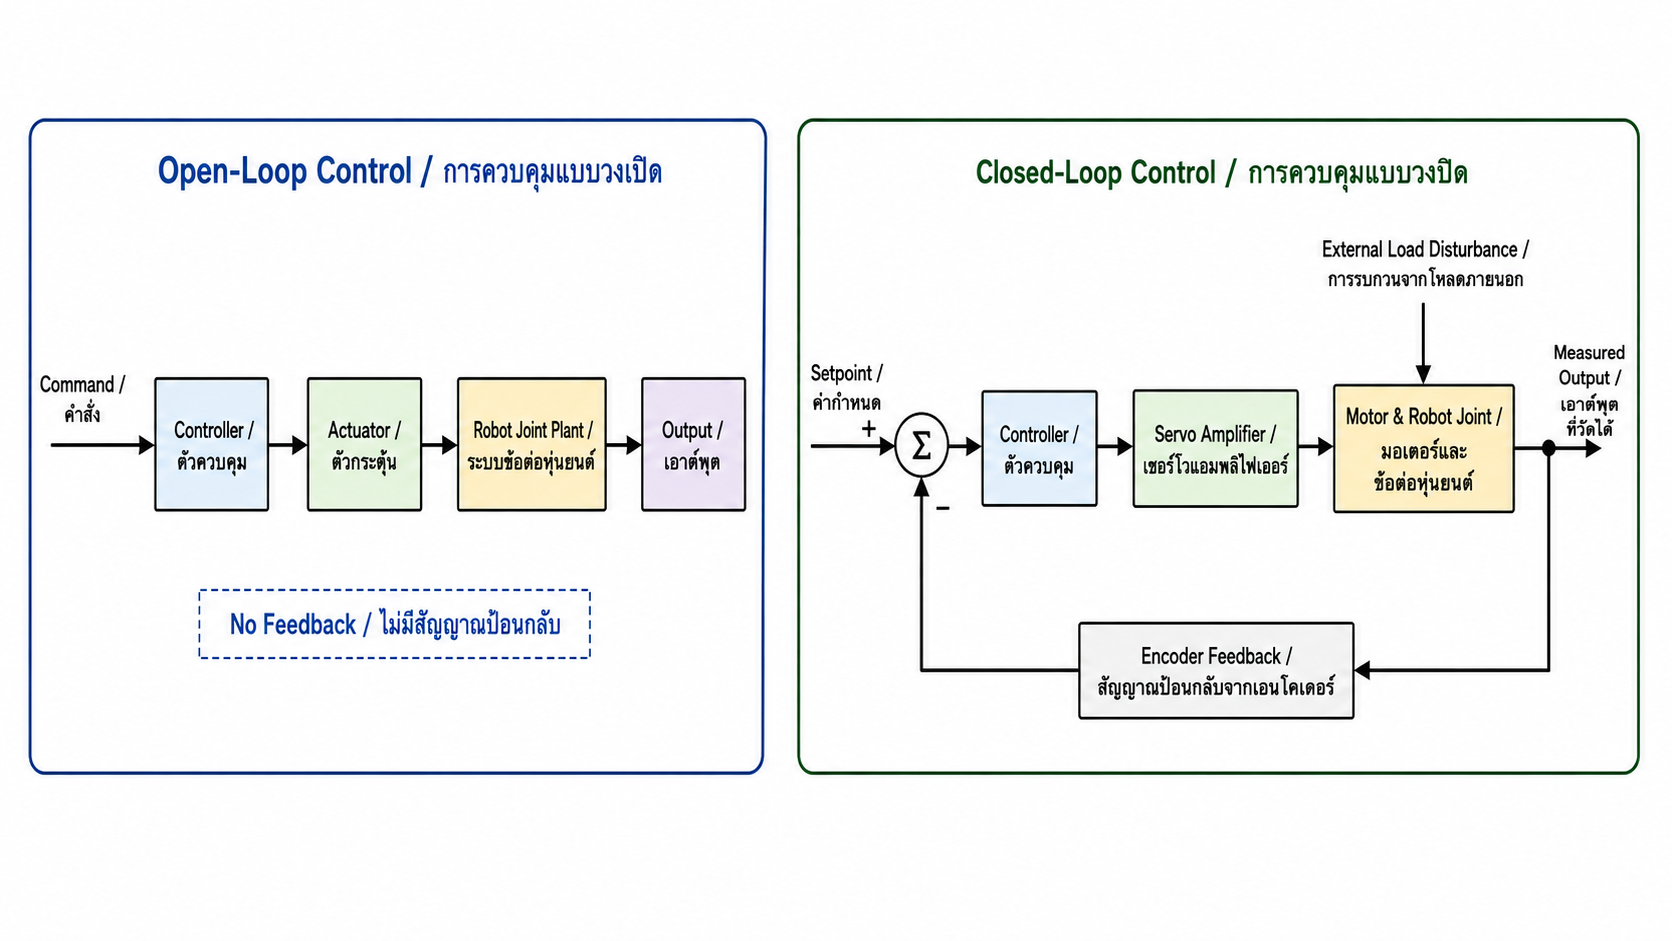
\includegraphics[width=0.8\textwidth]{images/chapter6/figure-01.png}
    \caption{การเปรียบเทียบระบบควบคุมวงเปิดและวงปิด}
\end{figure}



\subsubsection{ตัวชี้วัดสมรรถนะของผลตอบสนอง}

เมื่อให้คำสั่ง Step ระบบวงปิดมักประเมินด้วยตัวชี้วัดต่อไปนี้

\begin{enumerate}
    \item \textbf{Rise Time ($t_r$):} เวลาที่ผลตอบสนองเพิ่มจากค่าต่ำไปยังช่วงใกล้ค่าปลายทาง เกณฑ์อาจใช้ 10–90\% หรือเกณฑ์อื่น จึงต้องระบุให้ชัด
    \item \textbf{Peak Time ($t_p$):} เวลาที่เกิดค่าสูงสุดครั้งแรก
    \item \textbf{Maximum Overshoot ($M_p$):} ร้อยละที่ผลตอบสนองสูงเกินค่าปลายทาง
    \item \textbf{Settling Time ($t_s$):} เวลาที่ผลตอบสนองเข้าสู่และคงอยู่ในแถบ เช่น $\pm2\%$ หรือ $\pm5\%$
    \item \textbf{Steady-state Error ($e_{ss}$):} Error ที่เหลือเมื่อระบบเข้าสู่สภาวะคงตัว
    \item \textbf{Bandwidth:} ช่วงความถี่ที่ระบบสามารถติดตามคำสั่งหรือปฏิเสธ Disturbance ได้ตามเกณฑ์
    \item \textbf{Stability Margin:} ระยะเผื่อก่อนระบบเข้าสู่ภาวะไม่เสถียร เช่น Gain Margin และ Phase Margin
\end{enumerate}

ค่าพุ่งเกินคำนวณได้โดย

\[
M_p(\%)=\frac{y_{max}-y_{ss}}{y_{ss}}\times100
\]

โดย $y_{max}$ คือค่าสูงสุด และ $y_{ss}$ คือค่าปลายทาง

\paragraph{ตัวอย่างที่ 6.2 การคำนวณ Overshoot}

\textbf{ตัวอย่างเพิ่มเติมเพื่อการเรียนรู้}

ระบบตำแหน่งได้รับคำสั่ง $90^\circ$ วัดค่าสูงสุดได้ $99^\circ$ และเข้าสู่ค่าคงตัว $90^\circ$

\[
M_p=\frac{99-90}{90}\times100=10\%
\]

ผลตอบสนองมี Overshoot เท่ากับ 10\% หากงานเป็นการประกอบใกล้ชิ้นส่วนอื่น ค่า Overshoot นี้อาจมากเกินไปแม้ค่าปลายทางถูกต้อง จึงต้องประเมินทั้ง Transient Response และข้อจำกัดของพื้นที่ทำงาน



\subsubsection{การควบคุมแบบ PID}

ตัวควบคุม PID แบบต่อเนื่องมีรูป

\[
u(t)=K_p e(t)+K_i\int_0^t e(\tau)\,d\tau+K_d\frac{de(t)}{dt}
\]

โดย

\begin{itemize}
    \item $u(t)$ คือคำสั่งควบคุม เช่น กระแสอ้างอิง แรงบิดอ้างอิง หรือความเร็วอ้างอิง
    \item $e(t)$ คือ Error
    \item $K_p$ คือ Proportional Gain
    \item $K_i$ คือ Integral Gain
    \item $K_d$ คือ Derivative Gain
\end{itemize}

หน่วยของ Gain ขึ้นกับหน่วยของ $u$ และ $e$ ตัวอย่างเช่น หาก $u$ มีหน่วยโวลต์และ $e$ มีหน่วยเรเดียน จะได้ $K_p$ หน่วยโวลต์ต่อเรเดียน $K_i$ หน่วยโวลต์ต่อเรเดียนต่อวินาที และ $K_d$ หน่วยโวลต์วินาทีต่อเรเดียน

ในโดเมนลาปลาซ เมื่อสมมติค่าเริ่มต้นเป็นศูนย์

\[
C(s)=K_p+\frac{K_i}{s}+K_ds
\]

\paragraph{7.4.1 พจน์สัดส่วน}

พจน์สัดส่วนสร้างคำสั่งตาม Error ปัจจุบัน

\[
u_P(t)=K_pe(t)
\]

การเพิ่ม $K_p$ มักทำให้ระบบตอบสนองเร็วขึ้นและลด Error แต่หากสูงเกินไปอาจเพิ่ม Overshoot การสั่น และความไวต่อ Noise หรือความหน่วง

\paragraph{7.4.2 พจน์ปริพันธ์}

พจน์ปริพันธ์สะสม Error ตามเวลา

\[
u_I(t)=K_i\int_0^t e(\tau)\,d\tau
\]

จุดเด่นคือกำจัด Steady-state Error สำหรับระบบและคำสั่งบางประเภท แต่ทำให้ Phase Lag เพิ่มและอาจเกิด Overshoot มากขึ้น หาก Actuator อิ่มตัวแต่ Integrator ยังสะสม Error จะเกิด \textbf{Integral Windup}

แนวทางลด Windup ได้แก่

\begin{itemize}
    \item จำกัดค่าของ Integral State
    \item หยุดสะสมเมื่อ Output Saturate และ Error มีทิศทางเพิ่ม Saturation
    \item ใช้ Back-calculation Anti-windup
    \item จำกัดคำสั่งและความเร่งก่อนเข้าสู่ PID
\end{itemize}

\paragraph{7.4.3 พจน์อนุพันธ์}

พจน์อนุพันธ์ตอบสนองต่ออัตราการเปลี่ยนแปลงของ Error

\[
u_D(t)=K_d\frac{de(t)}{dt}
\]

พจน์นี้ช่วยเพิ่ม Damping และลด Overshoot ได้ในหลายระบบ แต่ไวต่อ Noise จึงมักใช้ Derivative Filter แทนอนุพันธ์อุดมคติ เช่น

\[
C_D(s)=K_d\frac{Ns}{s+N}
\]

หรือทำ Derivative จากค่าที่วัดแทน Error เพื่อลด Derivative Kick เมื่อ Setpoint เปลี่ยนฉับพลัน

\paragraph{7.4.4 ผลโดยทั่วไปของการปรับ Gain}

\begin{table}[htbp]
    \centering
    \begin{tabular}{l l l l}
        \hline
        \textbf{ตัวแปรสมรรถนะ} & \textbf{เพิ่ม $K_p$} & \textbf{เพิ่ม $K_i$} & \textbf{เพิ่ม $K_d$} \\
        \hline
        Rise Time & มักลดลง & อาจลดลงเล็กน้อย & เปลี่ยนเล็กน้อย \\
        Overshoot & มักเพิ่มขึ้น & มักเพิ่มขึ้น & มักลดลงเมื่อกรองเหมาะสม \\
        Settling Time & อาจเพิ่มหรือลด & มักเพิ่มหากเกิดการสั่น & มักลดจาก Damping ที่เพิ่ม \\
        Steady-state Error & ลดลง & สามารถกำจัดได้ในเงื่อนไขที่เหมาะสม & ไม่กำจัดโดยตรง \\
        Noise Sensitivity & เพิ่มได้เมื่อ Gain สูง & ไวต่อ Bias ระยะยาว & สูง โดยเฉพาะ Noise ความถี่สูง \\
        Stability Margin & อาจลดลง & มักลดลง & อาจดีขึ้นในช่วงที่ออกแบบเหมาะสม \\
        \hline
    \end{tabular}
\end{table}

\begin{quote}
\textbf{ข้อควรระวัง:} ตารางนี้เป็นแนวโน้มทั่วไป ไม่ใช่กฎตายตัว ผลจริงขึ้นกับ Plant, Sampling Time, Filter, Saturation และโครงสร้างตัวควบคุม
\end{quote}

\paragraph{7.4.5 การปรับ PID แบบเป็นขั้นตอน}

แนวทางเชิงปฏิบัติสำหรับห้องทดลองมีดังนี้

\begin{enumerate}
    \item ตรวจสอบทิศทาง Feedback ให้ถูกต้อง หากกลับขั้วระบบจะเป็น Positive Feedback
    \item จำกัด Output, Speed และ Travel ให้อยู่ในระดับปลอดภัย
    \item เริ่มจาก $K_i=0$ และ $K_d=0$
    \item เพิ่ม $K_p$ ทีละน้อยจนตอบสนองเร็วแต่ยังไม่สั่นต่อเนื่อง
    \item เพิ่ม $K_i$ เพื่อกำจัด Error คงตัว พร้อมติดตาม Overshoot และ Windup
    \item เพิ่ม $K_d$ หรือ Damping Term เพื่อปรับ Transient Response หากสัญญาณวัดมี Noise ต่ำพอ
    \item ทดสอบหลาย Setpoint และหลายโหลด ไม่ใช้ผลจากจุดทำงานเดียว
    \item บันทึก Rise Time, Overshoot, Settling Time, Error และ Peak Control Effort
    \item ตรวจอุณหภูมิ กระแสสูงสุด และ Alarm ของ Drive
    \item ยืนยันผลด้วยการทำซ้ำและกำหนดเกณฑ์ยอมรับ
\end{enumerate}

\paragraph{ตัวอย่างที่ 6.3 การคำนวณเอาต์พุต PID ณ ขณะหนึ่ง}

\textbf{ตัวอย่างเพิ่มเติมเพื่อการเรียนรู้}

กำหนด $K_p=2.0$, $K_i=0.8\ \text{s}^{-1}$, $K_d=0.1\ \text{s}$ ณ เวลาหนึ่งมี Error $e=0.5$ หน่วย Integral Error เท่ากับ $0.3\ \text{unit·s}$ และอัตราการเปลี่ยน Error เท่ากับ $-0.4\ \text{unit/s}$

\[
u=K_pe+K_i\int e\,dt+K_d\frac{de}{dt}
\]

\[
u=2.0(0.5)+0.8(0.3)+0.1(-0.4)
\]

\[
u=1.00+0.24-0.04=1.20
\]

คำตอบคือ $u=1.20$ หน่วยคำสั่ง พจน์ D มีค่าเป็นลบเพราะ Error กำลังลดลง จึงช่วยชะลอการเข้าใกล้ Setpoint และลดแนวโน้ม Overshoot

\paragraph{7.4.6 PID แบบดิจิทัล}

Robot Controller และ Servo Drive ใช้ตัวควบคุมดิจิทัล จึงคำนวณตามรอบ Sampling Time $T_s$ รูปแบบอย่างง่ายคือ

\[
I[k]=I[k-1]+K_iT_se[k]
\]

\[
D[k]=K_d\frac{e[k]-e[k-1]}{T_s}
\]

\[
u[k]=K_pe[k]+I[k]+D[k]
\]

เมื่อ $T_s$ เปลี่ยน ผลของพจน์ I และ D จะเปลี่ยนตาม หากย้ายค่าพารามิเตอร์ระหว่าง Controller ที่ใช้สูตรภายในต่างกัน ต้องตรวจสอบนิยาม Gain ไม่ควรคัดลอกตัวเลขโดยตรงโดยไม่อ่านคู่มือ

%\paragraph{รูปที่ 6.2 PID Response Curves}

% [รูปที่ 6.2: ผลกระทบของค่า PID ต่อ Step Response]
% ประเภทภาพ: Graph
% ตำแหน่งที่แนะนำ: หลังหัวข้อ 7.4
% วัตถุประสงค์การเรียนรู้: แสดงแนวโน้มของ Rise Time, Overshoot, Settling Time และ Steady-state Error เมื่อปรับ Gain
% คำอธิบายภาพ: กราฟสี่ช่องหรือกราฟซ้อนที่เปรียบเทียบ Base Response กับกรณีเพิ่ม Kp, เพิ่ม Ki และเพิ่ม Kd โดยใช้เส้น Setpoint เดียวกัน และกำกับว่าเป็นแนวโน้มเชิงคุณภาพ
% องค์ประกอบที่ต้องมี: แกนเวลา แกนผลตอบสนอง เส้น Setpoint จุด Overshoot และแถบ Settling
% ข้อความหรือป้ายกำกับ: Base, Higher Kp, Higher Ki, Higher Kd, Setpoint, Overshoot, Settling Band
% ภาษาของป้ายกำกับ: ไทยและอังกฤษ
% สัดส่วนภาพ: 16:9
% Graph Generation Prompt: Create an engineering textbook graph illustrating qualitative PID gain effects on a normalized unit-step response. Use four clearly labeled panels: baseline, increased Kp, increased Ki, and increased Kd. Show normalized output y(t) from 0 to 1.5 and time from 0 to 5 seconds. Include a horizontal setpoint at 1.0, mark overshoot and a ±2 percent settling band, and state that curves are conceptual and plant-dependent. Bilingual Thai-English labels, clean white background, 16:9.
% Alt Text: กราฟเชิงแนวคิดแสดงว่าการเพิ่ม Kp และ Ki มักเพิ่มความเร็วและ Overshoot ขณะที่ Kd เพิ่ม Damping แต่ผลจริงขึ้นกับระบบ

\begin{figure}[htbp]
    \centering
    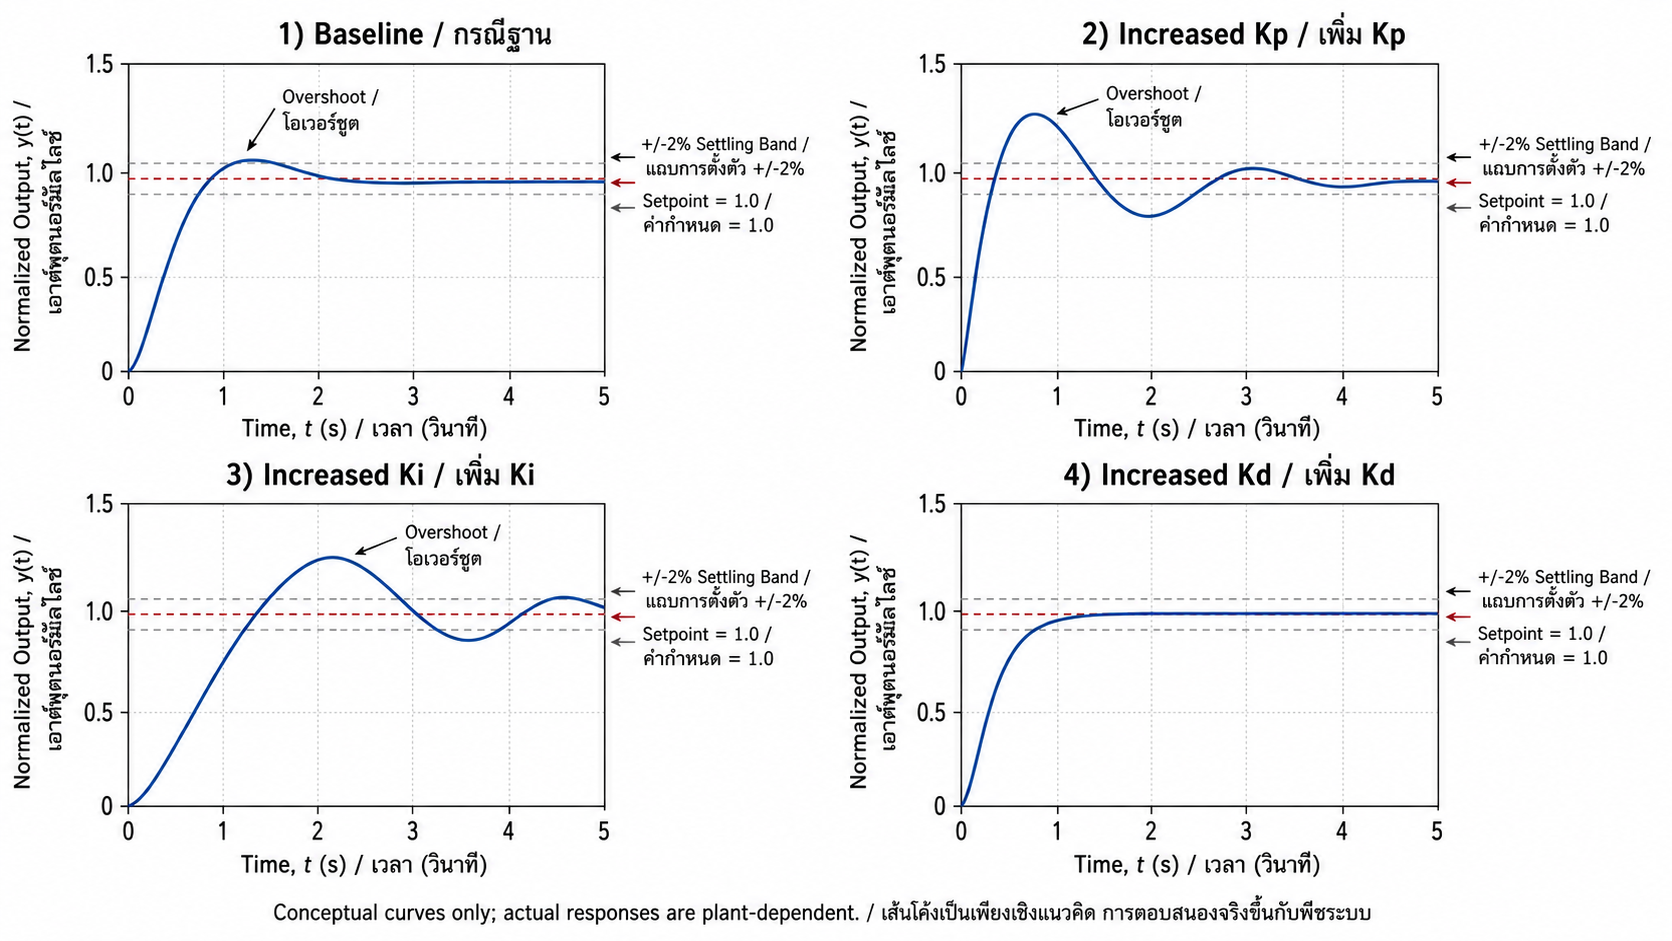
\includegraphics[width=0.8\textwidth]{images/chapter6/figure-02.png}
    \caption{ผลกระทบของค่า PID ต่อ Step Response}
\end{figure}



\subsubsection{การควบคุมตำแหน่ง ความเร็ว และแรงบิด}

Servo Drive สมัยใหม่มักรองรับหลายโหมดควบคุม แต่ละโหมดมีตัวแปรควบคุมและการใช้งานแตกต่างกัน

\paragraph{7.5.1 Position Control}

Position Control มีเป้าหมายให้ตำแหน่งจริง $q(t)$ ติดตามตำแหน่งคำสั่ง $q_d(t)$

\[
e_q(t)=q_d(t)-q(t)
\]

คำสั่งจาก Position Controller มักเป็นความเร็วอ้างอิงหรือแรงบิดอ้างอิง ขึ้นกับสถาปัตยกรรม ตัวอย่างงาน ได้แก่

\begin{itemize}
    \item Point-to-Point Motion
    \item Pick and Place
    \item งานประกอบ
    \item งานเชื่อมตามเส้นทาง
    \item การวางชิ้นงานที่ต้องการ Repeatability สูง
\end{itemize}

Position Control ต้องพิจารณา Motion Profile เพื่อจำกัดความเร็ว ความเร่ง และ Jerk หากเปลี่ยน Setpoint แบบ Step โดยตรง อาจทำให้คำสั่งแรงบิดสูงเกินขีดจำกัด

\paragraph{7.5.2 Speed Control}

Speed Control ให้ความเร็วจริง $\omega(t)$ ติดตามค่าคำสั่ง $\omega_d(t)$

\[
e_\omega(t)=\omega_d(t)-\omega(t)
\]

โหมดนี้ใช้ใน Conveyor, Spindle, Roll Feed และเป็นวงรอบภายในของ Position Control ความเร็วอาจคำนวณจาก Encoder โดยการหาความแตกต่างของตำแหน่งตามเวลา จึงต้องกรอง Noise โดยไม่เพิ่ม Delay มากเกินไป

\paragraph{7.5.3 Torque Control}

ในมอเตอร์ AC Servo ที่ใช้ Field-Oriented Control แรงบิดมีความสัมพันธ์โดยประมาณกับกระแสแกน $q$

\[
\tau_m=K_t i_q
\]

โดย $\tau_m$ คือแรงบิดมอเตอร์ หน่วย N·m, $K_t$ คือ Torque Constant หน่วย N·m/A และ $i_q$ คือกระแสสร้างแรงบิด หน่วย A

Torque Control เหมาะกับ

\begin{itemize}
    \item Force Control และ Contact Task
    \item Press-fit
    \item Screwdriving
    \item Tension Control
    \item Collision Detection บางรูปแบบ
    \item Gravity Compensation
\end{itemize}

อย่างไรก็ตาม แรงบิดมอเตอร์ไม่เท่ากับแรงที่ End Effector โดยตรง เพราะยังมีอัตราทด ประสิทธิภาพ แรงเสียดทาน และพลวัตของกลไก

หากละเลยการสูญเสียและใช้ Jacobian ความสัมพันธ์ระหว่าง Joint Torque กับ Wrench ที่ปลายแขนเขียนได้เป็น

\[
\boldsymbol{\tau}=\mathbf{J}^T(\mathbf{q})\mathbf{F}
\]

โดย $\boldsymbol{\tau}$ เป็นเวกเตอร์แรงบิดข้อต่อ และ $\mathbf{F}$ เป็นเวกเตอร์แรงและโมเมนต์ที่ End Effector

\paragraph{7.5.4 ตารางเลือกโหมดควบคุม}

\begin{table}[htbp]
    \centering
    \small
    \begin{tabularx}{\textwidth}{@{}L{0.12\textwidth} L{0.17\textwidth} L{0.14\textwidth} X X L{0.14\textwidth}@{}}
        \hline
        \textbf{โหมด} & \textbf{ตัวแปรป้อนกลับหลัก} & \textbf{คำสั่งหลัก} & \textbf{จุดเด่น} & \textbf{ข้อควรระวัง} & \textbf{ตัวอย่างงาน} \\
        \hline
        Position & ตำแหน่ง Encoder & Position/Trajectory & แม่นยำ เหมาะกับการเคลื่อนตามจุด & ต้องจำกัด Motion Profile & Pick and Place \\
        Speed & ความเร็วที่วัดหรือประมาณ & Speed & รักษาความเร็วสม่ำเสมอ & Noise จากการคำนวณความเร็ว & Conveyor, Spindle \\
        Torque & Current/Torque Estimate & Torque/Current & ควบคุมแรงสัมผัสได้รวดเร็ว & ต้องจำกัดแรงและจัดการ Gravity/Friction & Press-fit, Tension \\
        \hline
    \end{tabularx}
\end{table}



\subsubsection{โครงสร้างวงรอบซ้อนของ Servo Axis}

ระบบ Servo อุตสาหกรรมมักใช้วงรอบซ้อนดังนี้

\begin{center}
Position Command
$\downarrow$ \\
Position Controller -> Speed Command
$\downarrow$ \\
Speed Controller -> Torque/Current Command
$\downarrow$ \\
Current Controller -> PWM Inverter -> Servo Motor -> Robot Joint
$\downarrow$ \\
Current Sensor      Encoder Speed    Encoder Position
\end{center}

หลักสำคัญคือวงรอบด้านในต้องเร็วกว่าและคงตัวก่อน จึงออกแบบวงรอบด้านนอกได้ โดยทั่วไป

\begin{itemize}
    \item Current Loop เร็วที่สุด
    \item Speed Loop ช้ากว่า Current Loop
    \item Position Loop ช้าที่สุด
\end{itemize}

อัตราส่วน Bandwidth ที่เหมาะสมขึ้นกับระบบและผู้ผลิต ไม่ควรใช้ตัวเลขตายตัว แต่แนวปฏิบัติคือแยก Bandwidth แต่ละวงให้ห่างพอเพื่อลดปฏิสัมพันธ์

หากกำหนด Bandwidth โดยประมาณเป็น $f_i$, $f_v$ และ $f_p$ สำหรับ Current, Velocity และ Position Loop ตามลำดับ ควรมี

\[
f_i>f_v>f_p
\]

แนวทางเริ่มต้นเพื่อการศึกษาอาจใช้

\[
f_i\approx 5f_v, \qquad f_v\approx 5f_p
\]

แต่ต้องยืนยันกับ Plant จริงและคู่มือ Drive

\paragraph{ตัวอย่างที่ 6.4 การกำหนด Bandwidth เริ่มต้น}

\textbf{ตัวอย่างเพิ่มเติมเพื่อการเรียนรู้}

กำหนด Current Loop Bandwidth $f_i=1000\ \text{Hz}$ ต้องการกำหนดค่าเริ่มต้นของ Speed และ Position Loop ด้วยอัตราส่วน 5:1

\[
f_v=\frac{1000}{5}=200\ \text{Hz}
\]

\[
f_p=\frac{200}{5}=40\ \text{Hz}
\]

ค่าดังกล่าวเป็นเพียงจุดเริ่มต้น การใช้งานจริงต้องพิจารณา Resonance ของกลไก Sampling Frequency ความแข็งของ Gearbox และ Filter

\paragraph{7.6.1 Following Error}

Following Error คือผลต่างระหว่างตำแหน่งคำสั่งกับตำแหน่งจริง

\[
e_f(t)=q_d(t)-q(t)
\]

Robot Controller มักกำหนดขีดจำกัด Following Error หากเกินค่าที่กำหนดจะเกิด Alarm เพื่อป้องกันการเคลื่อนที่ผิดปกติ สาเหตุอาจมาจาก

\begin{itemize}
    \item โหลดมากเกินไป
    \item กลไกติดขัด
    \item Gain ต่ำหรือสูงไม่เหมาะสม
    \item Encoder Fault
    \item Motor Phase หรือ Brake ผิดปกติ
    \item Command Profile รุนแรงเกินไป
\end{itemize}

%\paragraph{รูปที่ 6.3 Cascade Control Block Diagram}

% [รูปที่ 6.3: โครงสร้างวงรอบซ้อน Position–Speed–Current]
% ประเภทภาพ: Block Diagram
% ตำแหน่งที่แนะนำ: หลังหัวข้อ 7.6
% วัตถุประสงค์การเรียนรู้: อธิบายความสัมพันธ์ของวงรอบตำแหน่ง ความเร็ว และกระแสใน Servo Drive
% คำอธิบายภาพ: แสดง Position Controller สร้าง Speed Reference, Speed Controller สร้าง Current/Torque Reference และ Current Controller ควบคุม PWM Inverter พร้อม Feedback จาก Encoder และ Current Sensor
% องค์ประกอบที่ต้องมี: Position command, Position loop, Speed loop, Current loop, PWM inverter, servo motor, gearbox, robot joint, encoder, current sensors, bandwidth labels
% ข้อความหรือป้ายกำกับ: Outer Loop, Inner Loop, Fastest Loop, Position Feedback, Speed Feedback, Current Feedback
% ภาษาของป้ายกำกับ: ไทยและอังกฤษ
% สัดส่วนภาพ: 16:9
% Image Generation Prompt: Detailed clean cascade control block diagram for an industrial robot servo axis. Show position command to position controller, speed command to speed controller, torque/current command to current controller, PWM inverter, servo motor, gearbox, and robot joint. Include encoder position feedback, calculated speed feedback, phase current sensors, and arrows. Label current loop as fastest, speed loop as intermediate, position loop as outer and slowest. Engineering textbook vector style, bilingual Thai-English labels, white background, 16:9.
% Alt Text: แผนภาพวงรอบซ้อนที่ Current Loop อยู่ด้านในสุด ตามด้วย Speed Loop และ Position Loop อยู่ด้านนอก

\begin{figure}[htbp]
    \centering
    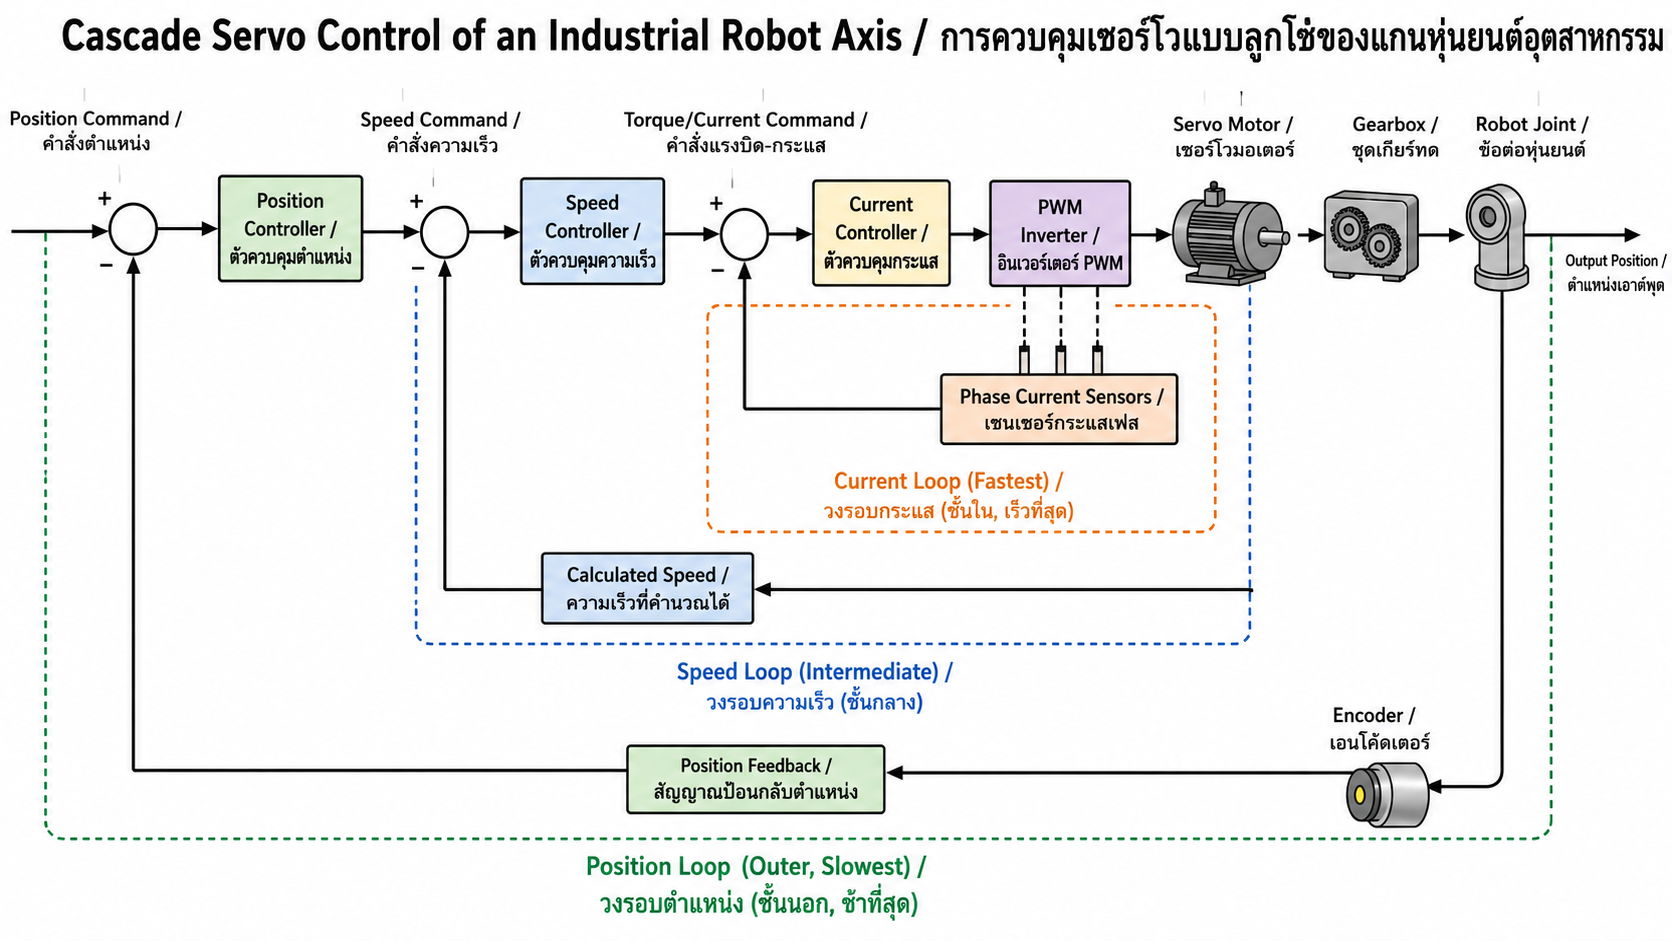
\includegraphics[width=0.8\textwidth]{images/chapter6/figure-03.png}
    \caption{โครงสร้างวงรอบซ้อน Position–Speed–Current}
\end{figure}



\subsubsection{การควบคุมใน Joint Space และ Cartesian Space}

\paragraph{7.7.1 Joint Space Control}

Joint Space Control ควบคุมตัวแปรข้อต่อโดยตรง

\[
\mathbf{q}=\begin{bmatrix}q_1&q_2&\cdots&q_n\end{bmatrix}^T
\]

สำหรับหุ่นยนต์ข้อต่อหมุน $q_i$ คือมุม สำหรับข้อต่อเลื่อน $q_i$ คือระยะทาง วิธีนี้เหมาะกับ Point-to-Point Motion เพราะสามารถวางแผนโปรไฟล์ของแต่ละแกนแล้วให้ทุกแกนถึงเป้าหมายพร้อมกัน

\textbf{ข้อดี}

\begin{itemize}
    \item สอดคล้องกับตัวแปรที่ Servo Controller วัดโดยตรง
    \item คำนวณง่ายกว่า Cartesian Control
    \item เหมาะกับการเคลื่อนที่ที่ไม่กำหนดเส้นทางปลายแขนอย่างเข้มงวด
\end{itemize}

\textbf{ข้อจำกัด}

\begin{itemize}
    \item เส้นทางของ End Effector อาจไม่เป็นเส้นตรง
    \item ต้องใช้ Inverse Kinematics เพื่อแปลงเป้าหมาย Cartesian เป็น Joint Coordinates
    \item ใกล้ Singular Configuration การเปลี่ยนตำแหน่งเล็กน้อยอาจต้องใช้ความเร็วข้อต่อสูง
\end{itemize}

\paragraph{7.7.2 Cartesian Space Control}

กำหนด Pose ของ End Effector เป็น

\[
\mathbf{x}=\begin{bmatrix}x&y&z&\phi&\theta&\psi\end{bmatrix}^T
\]

ความสัมพันธ์เชิงความเร็วคือ

\[
\dot{\mathbf{x}}=\mathbf{J}(\mathbf{q})\dot{\mathbf{q}}
\]

หาก Jacobian มี Inverse ที่เหมาะสม

\[
\dot{\mathbf{q}}=\mathbf{J}^{-1}(\mathbf{q})\dot{\mathbf{x}}
\]

สำหรับหุ่นยนต์ที่ไม่เป็นเมทริกซ์จัตุรัสหรืออยู่ใกล้ Singular มักใช้ Pseudoinverse

\[
\dot{\mathbf{q}}=\mathbf{J}^{\dagger}(\mathbf{q})\dot{\mathbf{x}}
\]

Cartesian Control เหมาะกับงานที่ต้องควบคุมเส้นทางหรือแรงในพิกัดงาน เช่น เชื่อม เจียร ขัดผิว และประกอบชิ้นส่วน

\paragraph{7.7.3 Singularities}

Singularity คือสภาวะที่หุ่นยนต์สูญเสียความสามารถในการสร้างความเร็วหรือแรงในบางทิศทาง หรือจำเป็นต้องใช้ความเร็วข้อต่อสูงมากเพื่อให้ได้ความเร็ว Cartesian ที่กำหนด ใกล้ Singularity ค่าของ $\mathbf{J}^{-1}$ อาจมีขนาดสูงและไวต่อ Noise

แนวทางจัดการ ได้แก่

\begin{itemize}
    \item หลีกเลี่ยงเส้นทางใกล้ Singularity
    \item จำกัด Joint Speed
    \item ใช้ Damped Least Squares Pseudoinverse
    \item เปลี่ยนท่าทางของ Tool หรือ Workpiece
    \item วางตำแหน่งฐานหุ่นยนต์ให้ Workspace เหมาะสม
\end{itemize}

\paragraph{7.7.4 Computed Torque Control}

พลวัตของหุ่นยนต์เขียนได้เป็น

\[
\mathbf{M}(\mathbf{q})\ddot{\mathbf{q}}+\mathbf{C}(\mathbf{q},\dot{\mathbf{q}})\dot{\mathbf{q}}+\mathbf{g}(\mathbf{q})+\mathbf{f}(\dot{\mathbf{q}})=\boldsymbol{\tau}
\]

โดย

\begin{itemize}
    \item $\mathbf{M}(\mathbf{q})$ คือ Inertia Matrix
    \item $\mathbf{C}(\mathbf{q},\dot{\mathbf{q}})\dot{\mathbf{q}}$ คือ Coriolis และ Centrifugal Term
    \item $\mathbf{g}(\mathbf{q})$ คือ Gravity Term
    \item $\mathbf{f}(\dot{\mathbf{q}})$ คือ Friction
    \item $\boldsymbol{\tau}$ คือ Joint Torque
\end{itemize}

Computed Torque Control ใช้แบบจำลองชดเชย Nonlinear Dynamics แล้วกำหนด Tracking Error Dynamics ที่ต้องการ รูปหนึ่งคือ

\[
\boldsymbol{\tau}=\mathbf{M}(\mathbf{q})\left[\ddot{\mathbf{q}}_d+\mathbf{K}_d(\dot{\mathbf{q}}_d-\dot{\mathbf{q}})+\mathbf{K}_p(\mathbf{q}_d-\mathbf{q})\right]
+\mathbf{C}(\mathbf{q},\dot{\mathbf{q}})\dot{\mathbf{q}}+\mathbf{g}(\mathbf{q})
\]

เมื่อแบบจำลองแม่นยำ ระบบ Error จะมีพฤติกรรมใกล้เคียงระบบเชิงเส้นอันดับสอง แต่ความคลาดเคลื่อนของมวล Payload แรงเสียดทาน และความยืดหยุ่นทำให้ประสิทธิภาพลดลง จึงอาจต้องใช้ Robust หรือ Adaptive Compensation

\paragraph{ตัวอย่างที่ 6.5 Gravity Compensation ของข้อต่อเดียว}

\textbf{ตัวอย่างเพิ่มเติมเพื่อการเรียนรู้}

แขนข้อต่อเดียวมีมวลรวม $m=5\ \text{kg}$ จุดศูนย์กลางมวลอยู่ห่างแกน $l=0.25\ \text{m}$ และแขนทำมุม $\theta=60^\circ$ วัดจากแนวดิ่ง กำหนด $g=9.81\ \text{m/s}^2$

แรงบิดโน้มถ่วงคือ

\[
\tau_g=mgl\sin\theta
\]

\[
\tau_g=5(9.81)(0.25)\sin60^\circ
\]

\[
\tau_g\approx10.62\ \text{N·m}
\]

Controller ต้องสร้างแรงบิดอย่างน้อยประมาณ $10.62\ \text{N·m}$ เพื่อคงตำแหน่งในแบบจำลองอุดมคติ และต้องเผื่อแรงเสียดทาน การเร่ง และประสิทธิภาพชุดส่งกำลังในระบบจริง



\subsubsection{การเชื่อมต่อ PLC กับ Robot Controller}

PLC ทำหน้าที่ควบคุมลำดับงานระดับเซลล์ ขณะที่ Robot Controller จัดการ Motion Planning และ Servo Control การแบ่งหน้าที่ที่ชัดเจนช่วยลดความซับซ้อนและทำให้วินิจฉัยปัญหาง่าย

\paragraph{7.8.1 Digital I/O แบบเดินสายตรง}

ตัวอย่างสัญญาณจาก PLC ไป Robot Controller

\begin{itemize}
    \item Cycle Start
    \item Cycle Stop หรือ Hold
    \item Reset Fault
    \item Program Select Bits
    \item Part Present
    \item Fixture Clamped
    \item Permission to Enter
    \item Automatic Mode Request
\end{itemize}

ตัวอย่างสัญญาณจาก Robot Controller ไป PLC

\begin{itemize}
    \item Robot Ready
    \item Servo On Status
    \item Running
    \item Program Complete
    \item At Home
    \item At Maintenance Position
    \item Gripper Open/Closed
    \item Fault Present
    \item Fault Code Bits
\end{itemize}

\begin{quote}
\textbf{ข้อสำคัญด้านความปลอดภัย:} Emergency Stop, Guard Door และฟังก์ชัน Safety ต้องใช้วงจรหรือเครือข่ายที่มีระดับความปลอดภัยเหมาะสม เช่น Safety Relay, Safety PLC, Dual-channel Safety I/O หรือ Safety Protocol ตามการประเมินความเสี่ยง ไม่ควรนำ E-Stop ผ่าน Standard PLC I/O เพียงอย่างเดียว
\end{quote}

\paragraph{7.8.2 Source/Sink และ PNP/NPN}

การต่อ Digital I/O ต้องตรวจสอบชนิดเอาต์พุตและอินพุต

\begin{itemize}
    \item \textbf{PNP Output:} จ่ายแรงดันบวกให้โหลดเมื่อ ON มักเรียก Sourcing Output
    \item \textbf{NPN Output:} ดึงกระแสลง 0 V เมื่อ ON มักเรียก Sinking Output
\end{itemize}

หาก PLC และ Robot I/O ใช้ Logic ไม่เข้ากัน อาจใช้ Interposing Relay, Optocoupler หรือ Interface Module การต่อ Common Reference ผิดอาจทำให้สัญญาณไม่ทำงานหรือทำให้อุปกรณ์เสียหาย

\paragraph{7.8.3 Handshake Sequence}

การส่ง Pulse Start เพียงเส้นเดียวอาจทำให้เกิด Race Condition หรือคำสั่งสูญหาย จึงควรใช้ Handshake ตัวอย่างลำดับคือ

\begin{enumerate}
    \item PLC ตรวจสอบ Robot Ready และ Cell Safe
    \item PLC กำหนด Program Number
    \item PLC เปิดสัญญาณ Start Request
    \item Robot ตรวจ Program Number และตอบ Start Acknowledge
    \item PLC ปิด Start Request
    \item Robot ปิด Start Acknowledge และเริ่มทำงาน
    \item Robot เปิด Running
    \item เมื่อจบงาน Robot เปิด Complete
    \item PLC รับ Complete และปิดเงื่อนไขรอบงาน
    \item Robot ปิด Complete เมื่อได้รับ Acknowledge หรือเมื่อเงื่อนไข Reset ครบ
\end{enumerate}

ควรกำหนด Timeout ทุกขั้นตอน หากไม่ได้รับ Acknowledge ภายในเวลาที่กำหนด PLC ต้องเข้าสู่สถานะ Fault หรือ Recovery ที่ปลอดภัย

\paragraph{7.8.4 การเลือก Program ด้วย Bit}

หากใช้ $n$ บิต จะเลือกหมายเลขโปรแกรมได้สูงสุด

\[
N=2^n
\]

ตัวอย่างใช้ 4 บิตเลือกได้ 16 ค่า ตั้งแต่ 0 ถึง 15 แต่ควรกำหนดบางรหัสไว้สำหรับ No Program, Maintenance หรือ Invalid Code

\paragraph{ตัวอย่างที่ 6.6 การออกแบบ Program Select}

ต้องการเลือกโปรแกรมการผลิต 10 โปรแกรม

หา $n$ ที่ทำให้

\[
2^n\ge10
\]

เมื่อ $n=3$ จะได้ 8 ค่า ไม่เพียงพอ เมื่อ $n=4$ จะได้ 16 ค่า จึงต้องใช้ Program Select อย่างน้อย 4 บิต

\paragraph{7.8.5 Analog I/O}

Analog I/O ใช้ส่งค่าต่อเนื่อง เช่น

\begin{itemize}
    \item Speed Reference 0–10 V
    \item Force/Torque Reference ±10 V
    \item Process Value 4–20 mA
    \item Pressure หรือ Flow Feedback
\end{itemize}

ข้อดีของ 4–20 mA คือสามารถตรวจจับสายขาดได้เมื่อกระแสต่ำกว่า 4 mA และทน Noise ในระยะไกลได้ดีกว่าสัญญาณแรงดันในหลายสภาพแวดล้อม

การแปลงสเกลแบบเชิงเส้นจากกระแส $I$ ช่วง 4–20 mA ไปยังค่ากระบวนการ $x$ ช่วง $x_{min}$ ถึง $x_{max}$ คือ

\[
x=x_{min}+\frac{I-4}{16}(x_{max}-x_{min})
\]

\paragraph{ตัวอย่างที่ 6.7 การแปลง 4–20 mA เป็นแรงบิด}

Torque Sensor กำหนดช่วง 4–20 mA เท่ากับ 0–200 N·m วัดได้ 12 mA

\[
\tau=0+\frac{12-4}{16}(200-0)
\]

\[
\tau=100\ \text{N·m}
\]

%\paragraph{รูปที่ 6.4 Robot–PLC I/O Wiring}

% [รูปที่ 6.4: การต่อ PLC กับ Robot Controller ผ่าน Hard-wired I/O]
% ประเภทภาพ: Technical Illustration / Wiring Diagram
% ตำแหน่งที่แนะนำ: หลังหัวข้อ 7.8
% วัตถุประสงค์การเรียนรู้: แสดงการแยก Standard I/O, Analog I/O และ Safety Circuit
% คำอธิบายภาพ: PLC Standard Output ต่อไปยัง Robot Standard Input ผ่าน Interface Relay; Robot Output ต่อกลับ PLC Input; Analog 4–20 mA แยก Shield; E-Stop และ Guard Door ผ่าน Safety Relay หรือ Safety PLC แบบสองช่องสัญญาณไปยัง Safety Interface ของ Robot
% องค์ประกอบที่ต้องมี: 24 VDC supply, fuse, PLC I/O, robot controller I/O, terminal blocks, interposing relays, common 0 V, shield grounding, safety relay, dual-channel E-stop, guard switch
% ข้อความหรือป้ายกำกับ: Standard Control, Safety-rated Circuit, Do Not Route E-stop Through Standard I/O Only
% ภาษาของป้ายกำกับ: ไทยและอังกฤษ
% สัดส่วนภาพ: 16:9
% Image Generation Prompt: Safe educational wiring diagram of a PLC connected to an industrial robot controller. Show 24 VDC standard digital outputs and inputs through terminal blocks and interposing relays for Start, Reset, Ready, Running, Complete and Fault. Show a separate shielded 4–20 mA analog channel. Clearly separate a dual-channel emergency-stop and guard-door circuit through a safety relay or safety PLC to the robot safety interface. Include fuses, common 0 V, protective earth, cable shields, and warning that emergency stop must not rely on standard PLC I/O alone. Clean engineering textbook vector style, bilingual labels, white background, 16:9.
% Alt Text: แผนผังต่อสาย PLC กับ Robot Controller ที่แยกวงจรควบคุมปกติออกจากวงจร Safety แบบสองช่องสัญญาณ

\begin{figure}[htbp]
    \centering
    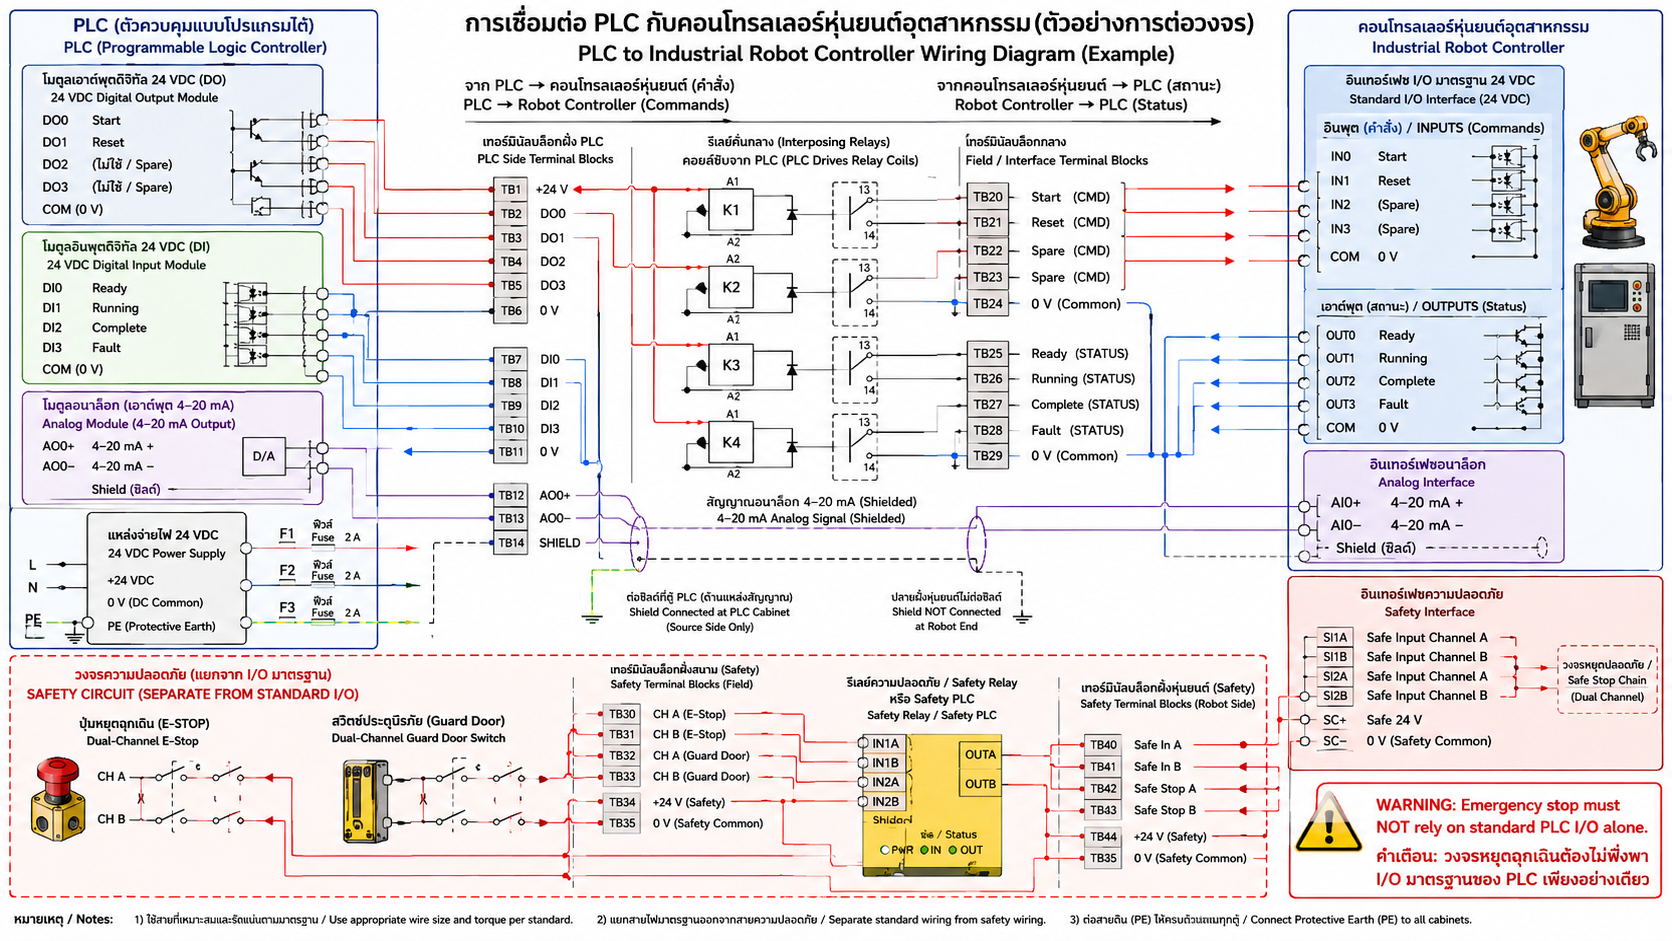
\includegraphics[width=0.8\textwidth]{images/chapter6/figure-04.png}
    \caption{การต่อ PLC กับ Robot Controller ผ่าน Hard-wired I/O}
\end{figure}



\subsubsection{ระดับการบูรณาการ Robot–PLC}

\begin{table}[htbp]
    \centering
    \small
    \begin{tabularx}{\textwidth}{@{}L{0.07\textwidth} L{0.15\textwidth} X L{0.13\textwidth} X X@{}}
        \hline
        \textbf{ระดับ} & \textbf{วิธีการ} & \textbf{ลักษณะข้อมูล} & \textbf{ความซับซ้อน} & \textbf{จุดเด่น} & \textbf{ข้อจำกัด} \\
        \hline
        1 & Hard-wired I/O & บิตสถานะและคำสั่ง & ต่ำ & เข้าใจง่าย แยกปัญหาง่าย & สายจำนวนมาก ข้อมูลจำกัด \\
        2 & Serial Fieldbus & Cyclic I/O และ Parameter บางส่วน & ปานกลาง & ลดสาย รองรับหลายอุปกรณ์ & Bandwidth และ Diagnostics จำกัดกว่าระบบใหม่ \\
        3 & Industrial Ethernet & Cyclic I/O, Acyclic, Diagnostics & ปานกลางถึงสูง & เร็ว ยืดหยุ่น จัดการข้อมูลมาก & ต้องออกแบบ Switch, Address และ Network Load \\
        4 & OPC UA / Middleware / ROS-Industrial & Semantic Data, Services, Integration & สูง & เชื่อมระดับเครื่องถึงระบบข้อมูล & ไม่แทน Hard Real-time Servo Loop หรือ Safety โดยอัตโนมัติ \\
        \hline
    \end{tabularx}
\end{table}

OPC UA เหมาะกับการแลกเปลี่ยนข้อมูลที่มีโครงสร้าง การวินิจฉัย Recipe และการเชื่อม MES/SCADA ส่วน ROS-Industrial สนับสนุนการเชื่อมอุปกรณ์หุ่นยนต์และความสามารถระดับสูง เช่น Perception และ Motion Planning แต่การนำไปใช้ในโรงงานยังต้องออกแบบ Layer สำหรับ Real-time, Safety และการบำรุงรักษาให้เหมาะสม



\subsubsection{7.10 แนวคิดพื้นฐานของการสื่อสารอุตสาหกรรม}

การประเมินเครือข่ายสำหรับงานควบคุมไม่ควรพิจารณาเพียงอัตราส่งข้อมูลเป็น Mbps แต่ต้องพิจารณาคุณลักษณะด้านเวลาและความน่าเชื่อถือด้วย

\paragraph{7.10.1 Throughput, Cycle Time, Latency และ Jitter}

\begin{itemize}
    \item \textbf{Link Speed:} อัตราสัญญาณของ Physical Link เช่น 100 Mbps หรือ 1 Gbps
    \item \textbf{Throughput:} ปริมาณข้อมูลใช้งานจริงต่อเวลา หลังหัก Overhead และช่วงเวลารอ
    \item \textbf{Cycle Time / Update Time:} เวลาที่ข้อมูล Process Data ถูกแลกเปลี่ยนครบหนึ่งรอบ
    \item \textbf{Latency:} เวลาจากเหตุการณ์ต้นทางจนข้อมูลมีผลที่ปลายทาง
    \item \textbf{Jitter:} ความแปรปรวนของ Cycle Time หรือ Latency
    \item \textbf{Determinism:} ความสามารถในการรับประกันว่าการสื่อสารเสร็จภายในกรอบเวลาที่กำหนด
\end{itemize}

เครือข่าย 1 Gbps อาจมี Latency ที่ไม่แน่นอนหากใช้สวิตช์หรือ Traffic ที่ไม่จัดการ ขณะที่เครือข่ายอัตราต่ำกว่าแต่ออกแบบ Scheduling แบบ Real-time อาจให้ Timing ที่คาดการณ์ได้มากกว่า

\paragraph{7.10.2 Cyclic และ Acyclic Communication}

\textbf{Cyclic Data} ใช้กับ I/O และคำสั่งควบคุมที่ต้องอัปเดตสม่ำเสมอ เช่น Robot Ready, Position Actual และ Torque Command

\textbf{Acyclic Data} ใช้กับ Parameter, Alarm History, Device Identification และ Diagnostic การส่ง Acyclic Traffic ต้องไม่รบกวน Cyclic Control เกินเกณฑ์

\paragraph{7.10.3 การประมาณงบประมาณเวลา}

เวลาตอบสนองรวมของระบบประมาณได้จาก

\[
T_{response}=T_{input}+T_{PLC}+T_{network,out}+T_{robot}+T_{network,in}+T_{output}
\]

โดยแต่ละพจน์อาจมีทั้งค่าเฉลี่ยและค่าสูงสุด การออกแบบงาน Interlock ควรใช้ Worst-case หรือค่าที่ผู้ผลิตรับรอง ไม่ใช้เพียงค่าที่วัดได้หนึ่งครั้ง

\paragraph{ตัวอย่างที่ 6.8 งบประมาณเวลาของ Handshake}

\textbf{ตัวอย่างเพิ่มเติมเพื่อการเรียนรู้}

ระบบมี Input Filter 4 ms, PLC Scan 8 ms, Network Update ไปและกลับด้านละ 4 ms, Robot Task Response 12 ms และ Output Module 4 ms

\[
T_{response}=4+8+4+12+4+4=36\ \text{ms}
\]

ดังนั้น Timeout 20 ms จะสั้นเกินไป แม้ระบบปกติอาจตอบเร็วกว่าในบางรอบ ควรเพิ่ม Margin ตาม Jitter และข้อกำหนดของกระบวนการ เช่นเลือก 100–200 ms สำหรับ Handshake ที่ไม่ใช่ Motion Synchronization ทั้งนี้ต้องทดสอบกับอุปกรณ์จริง



\subsubsection{7.11 แบบจำลอง OSI กับเครือข่ายอุตสาหกรรม}

OSI Model มี 7 ชั้น ได้แก่ Physical, Data Link, Network, Transport, Session, Presentation และ Application โปรโตคอลอุตสาหกรรมจำนวนมากไม่ได้ใช้ทุกชั้นแยกกันอย่างชัดเจน แต่แบบจำลองช่วยแยกปัญหาได้

\begin{table}[htbp]
    \centering
    \begin{tabular}{r l l}
        \hline
        \textbf{ชั้น OSI} & \textbf{หน้าที่โดยย่อ} & \textbf{ตัวอย่างประเด็นในระบบหุ่นยนต์} \\
        \hline
        7 Application & ความหมายของข้อมูลและบริการ & Modbus Function Code, CIP Object, PROFINET I/O Data \\
        6 Presentation & รูปแบบข้อมูล & Byte Order, Data Type, Encoding \\
        5 Session & การจัดการการเชื่อมต่อ & Connection State, Timeout \\
        4 Transport & การส่งปลายทางถึงปลายทาง & TCP, UDP \\
        3 Network & Addressing และ Routing & IP Address, Subnet, Router \\
        2 Data Link & Frame, MAC, Switching, Scheduling & Ethernet Frame, PROFINET RT, EtherCAT Processing \\
        1 Physical & สาย สัญญาณ Connector & RS-485, CAN, 100BASE-TX, Fiber \\
        \hline
    \end{tabular}
\end{table}

Modbus เป็น Application Protocol และสามารถทำงานเหนือ Serial Line หรือ TCP/IP ได้ จึงควรแยกคำว่า “Modbus” ออกจาก Physical Medium เช่น Modbus RTU over RS-485 และ Modbus TCP over Ethernet

%\paragraph{รูปที่ 6.5 OSI Model for Fieldbus}

% [รูปที่ 6.5: การวางโปรโตคอลอุตสาหกรรมบนแบบจำลอง OSI]
% ประเภทภาพ: Infographic / Layer Diagram
% ตำแหน่งที่แนะนำ: หลังหัวข้อ 7.11
% วัตถุประสงค์การเรียนรู้: ช่วยแยก Application Protocol ออกจาก Physical Layer และอธิบายสาเหตุที่โปรโตคอลต่างกันด้านเวลา
% คำอธิบายภาพ: แสดง OSI 7 ชั้น และวาง Modbus RTU, PROFIBUS DP, CANopen, Modbus TCP, EtherNet/IP, PROFINET และ EtherCAT โดยไม่สื่อว่าทุกโปรโตคอลใช้ทุกชั้นเต็มรูปแบบ
% องค์ประกอบที่ต้องมี: ชั้น 1–7, RS-485, CAN, Ethernet, TCP/UDP/IP, Application Objects, Cyclic I/O
% ข้อความหรือป้ายกำกับ: Application Layer, Transport, Network, Data Link, Physical; Serial Fieldbus; Industrial Ethernet
% ภาษาของป้ายกำกับ: ไทยและอังกฤษ
% สัดส่วนภาพ: 16:9
% Image Generation Prompt: Educational OSI model infographic for industrial robot communication. Show seven OSI layers and place representative technologies carefully: RS-485 and CAN at physical/data-link level, PROFIBUS DP and CANopen as fieldbus stacks, Modbus RTU over serial, Modbus TCP over TCP/IP and Ethernet, EtherNet/IP using CIP over standard Ethernet and TCP/UDP/IP, PROFINET with real-time data-link communication and standard Ethernet services, and EtherCAT processing Ethernet frames on the fly. Add a note that mappings are simplified and protocols do not necessarily implement every OSI layer separately. Bilingual Thai-English labels, clean engineering vector style, 16:9.
% Alt Text: อินโฟกราฟิก OSI 7 ชั้นที่เปรียบเทียบ Fieldbus และ Industrial Ethernet พร้อมแยก Physical Medium ออกจาก Application Protocol

\begin{figure}[htbp]
    \centering
    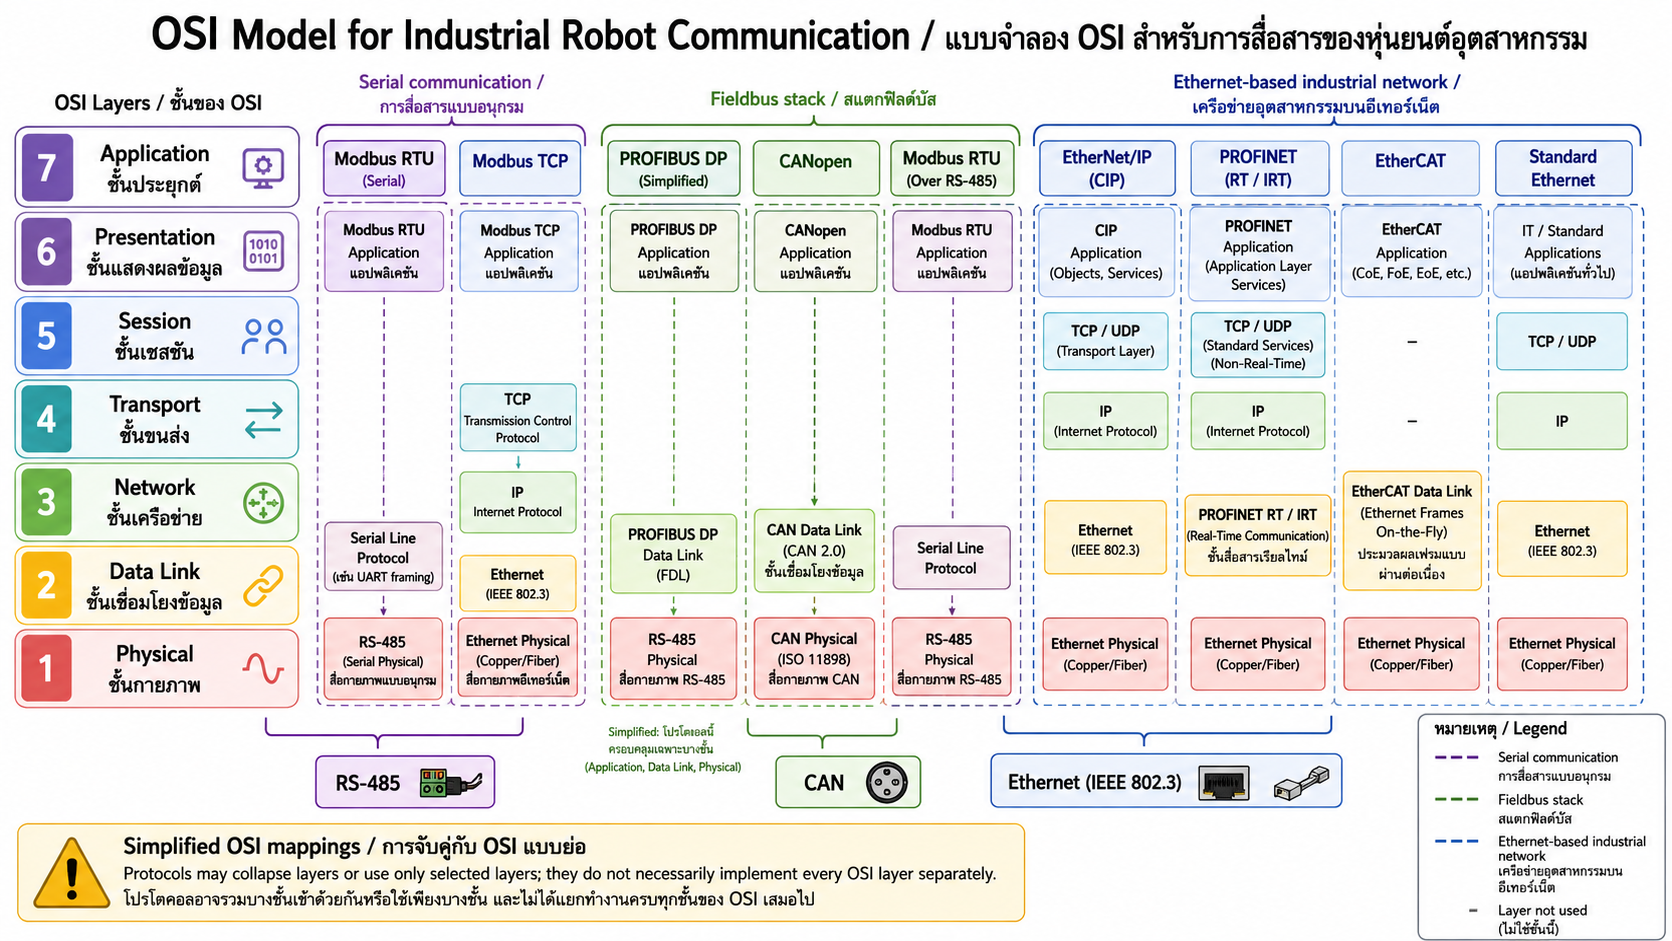
\includegraphics[width=0.8\textwidth]{images/chapter6/figure-05.png}
    \caption{การวางโปรโตคอลอุตสาหกรรมบนแบบจำลอง OSI}
\end{figure}



\subsubsection{Fieldbus ที่ใช้ในระบบหุ่นยนต์}

\paragraph{7.12.1 Modbus RTU}

Modbus RTU เป็นรูปแบบการส่งข้อความ Modbus บน Serial Line มักใช้ RS-485 แบบ Multi-drop โครงสร้างข้อมูลอิง Address และ Function Code เช่น Read Coils, Read Holding Registers และ Write Multiple Registers

\textbf{จุดเด่น}

\begin{itemize}
    \item โครงสร้างไม่ซับซ้อน
    \item มีอุปกรณ์รองรับจำนวนมาก
    \item เหมาะกับ I/O, Meter และอุปกรณ์ Legacy
\end{itemize}

\textbf{ข้อจำกัด}

\begin{itemize}
    \item ไม่มี Semantic Model ที่ละเอียด
    \item การวินิจฉัยและการกำหนดอุปกรณ์ขึ้นกับผู้ผลิต
    \item Timing ขึ้นกับ Baud Rate จำนวนอุปกรณ์ และ Polling Strategy
    \item ต้องจัดการ Byte/Word Order ให้ตรงกัน
\end{itemize}

อัตราส่ง 115.2 kbps พบได้ในอุปกรณ์หลายรุ่น แต่ไม่ใช่ค่าที่รับรองเหมือนกันทุกอุปกรณ์ ระยะสาย RS-485 ที่ยาวต้องลด Baud Rate ใช้สายและ Termination ที่เหมาะสม

\paragraph{7.12.2 PROFIBUS DP}

PROFIBUS DP เป็น Fieldbus สำหรับ Distributed I/O และอุปกรณ์ Automation รองรับอัตราส่งตั้งแต่ 9.6 kbps ถึง 12 Mbps ระยะทางต่อ Segment ลดลงเมื่อ Baud Rate สูงขึ้น ตัวอย่างตามแนวทาง PI คือประมาณ 1,200 m ที่อัตราต่ำ และประมาณ 100 m ที่ 3–12 Mbps เมื่อใช้สายทองแดง Type A ตามข้อกำหนด

\textbf{จุดเด่น}

\begin{itemize}
    \item ระบบนิเวศขนาดใหญ่ในโรงงานเดิม
    \item Cyclic I/O แบบ Master–Device
    \item มีไฟล์ GSD สำหรับ Configuration
\end{itemize}

\textbf{ข้อจำกัด}

\begin{itemize}
    \item ต้องติดตั้ง Termination และ Shield อย่างถูกต้อง
    \item การขยายหรือแก้ปัญหาต้องมีเครื่องมือเฉพาะ
    \item Bandwidth ต่ำกว่า Industrial Ethernet รุ่นใหม่
\end{itemize}

\paragraph{7.12.3 DeviceNet}

DeviceNet ใช้ Common Industrial Protocol (CIP) บน CAN เหมาะกับอุปกรณ์ระดับ Field Device อัตราส่งทั่วไป 125, 250 และ 500 kbps ระยะ Trunk ที่รองรับลดลงเมื่ออัตราส่งสูงขึ้น เช่นประมาณ 500 m ที่ 125 kbps และประมาณ 100 m ที่ 500 kbps ตามข้อกำหนดระบบ

\textbf{จุดเด่น}

\begin{itemize}
    \item ส่ง Power และ Communication ในสายระบบเดียวตามการออกแบบ
    \item ใช้ CIP Object Model
    \item เหมาะกับ Sensor, Valve Island และ Motor Starter รุ่นเดิม
\end{itemize}

\paragraph{7.12.4 CANopen}

CANopen เป็น Higher-layer Protocol บน CAN พัฒนาสำหรับ Embedded Control และ Motion-oriented Machine Control มี Object Dictionary, Process Data Object (PDO), Service Data Object (SDO), Network Management และ Device Profile

CiA 402 กำหนดพฤติกรรมมาตรฐานของ Servo Drive, Frequency Inverter และ Stepper Drive รวมถึง State Machine และ Operation Modes จึงพบใน Robot Joint, AGV และเครื่องจักรขนาดกะทัดรัด

\textbf{จุดเด่น}

\begin{itemize}
    \item มี Device Profile สำหรับ Motion
    \item Configurable และใช้ทรัพยากรไม่สูง
    \item เหมาะกับเครือข่ายภายในเครื่อง
\end{itemize}

\textbf{ข้อจำกัด}

\begin{itemize}
    \item Bandwidth ของ Classical CAN จำกัด
    \item ระยะสายสัมพันธ์กับ Bit Rate
    \item ต้องจัดสรร COB-ID และ PDO อย่างเป็นระบบ
\end{itemize}

\paragraph{7.12.5 CC-Link}

CC-Link แบบ Fieldbus ดั้งเดิมรองรับความเร็วได้ถึง 10 Mbps และระยะรวมสูงสุดขึ้นกับความเร็วและรูปแบบการติดตั้ง จึงไม่ควรตีความว่า 10 Mbps ใช้ได้พร้อมระยะ 1,200 m ในทุกกรณี ระบบนี้พบมากในระบบ Factory Automation ที่ใช้อุปกรณ์ Mitsubishi และผู้ผลิตในเอเชีย

ตระกูล CC-Link รุ่น Ethernet เช่น CC-Link IE Field ใช้ 1 Gbps ในรุ่นหลัก ขณะที่ CC-Link IE Field Network Basic ใช้ 100 Mbps เป็นข้อกำหนดขั้นต่ำและรองรับ Cyclic Communication ผ่าน Software Implementation

\paragraph{7.12.6 ตารางเปรียบเทียบ Fieldbus}

\begin{table}[htbp]
    \centering
    \small
    \begin{tabularx}{\textwidth}{@{}L{0.13\textwidth} L{0.14\textwidth} L{0.16\textwidth} L{0.18\textwidth} X X@{}}
        \hline
        \textbf{โปรโตคอล} & \textbf{Physical/พื้นฐาน} & \textbf{อัตราส่งตัวอย่าง} & \textbf{ระยะทางตัวอย่าง} & \textbf{การใช้งานเด่น} & \textbf{หมายเหตุ} \\
        \hline
        Modbus RTU & RS-485 & มักพบถึง 115.2 kbps & สูงสุดราว 1,200 m ที่อัตราต่ำและติดตั้งเหมาะสม & Meter, Remote I/O, Legacy & Timing ขึ้นกับ Polling และอุปกรณ์ \\
        PROFIBUS DP & RS-485 & 9.6 kbps–12 Mbps & 1,200 m ที่อัตราต่ำ; 100 m ที่ 3–12 Mbps ต่อ Segment & Distributed I/O, Drive & ใช้ Repeater เพิ่ม Segment ได้ \\
        DeviceNet & CAN/CIP & 125–500 kbps & ราว 500 m ที่ 125 kbps; 100 m ที่ 500 kbps & Sensor, Starter, Valve & ระยะ Spur และ Trunk ต้องตาม Design Guide \\
        CANopen & CAN & ถึง 1 Mbps สำหรับ Classical CAN & ราว 25–40 m ที่ 1 Mbps; ยาวขึ้นเมื่อ Bit Rate ต่ำ & Embedded Motion, Robot Joint & ใช้ CiA 402 ใน Drive \\
        CC-Link & RS-485-based fieldbus & ถึง 10 Mbps & ขึ้นกับ Baud Rate; สูงสุดรวมได้ราว 1,200 m ที่อัตราต่ำ & Mitsubishi FA & ต้องดูตารางความเร็ว–ระยะของรุ่น \\
        \hline
    \end{tabularx}
\end{table}

\begin{quote}
\textbf{การอ่านตาราง:} ค่าความเร็วและระยะทางเป็นค่าตัวอย่างเพื่อเปรียบเทียบ ไม่ใช่ค่ารับประกันสำหรับอุปกรณ์ทุกยี่ห้อ ต้องตรวจคู่มือ Interface Card, Cable และ Installation Guideline ก่อนออกแบบ
\end{quote}



\subsubsection{7.13 Industrial Ethernet}

Industrial Ethernet ใช้เทคโนโลยี Ethernet แต่เพิ่มกลไกและ Profile เพื่อให้เหมาะกับ Automation เช่น Cyclic I/O, Device Description, Diagnostics, Clock Synchronization, Redundancy และ Real-time Scheduling

\paragraph{7.13.1 EtherNet/IP}

EtherNet/IP ใช้ Common Industrial Protocol (CIP) บนมาตรฐาน Ethernet และ TCP/UDP/IP รองรับ Explicit Messaging สำหรับ Parameter/Configuration และ Implicit I/O Messaging สำหรับข้อมูลแบบคาบ ค่า Requested Packet Interval (RPI) กำหนดความถี่ในการแลกเปลี่ยน I/O แต่เวลาตอบสนองจริงขึ้นกับ PLC Task, Switch, Network Load และ Device

\textbf{จุดเด่น}

\begin{itemize}
    \item ใช้ Ethernet Infrastructure มาตรฐาน
    \item มี CIP Motion, CIP Safety, CIP Sync และ Device Profile
    \item พบมากในระบบ Rockwell Automation และ Robot หลายยี่ห้อ
\end{itemize}

\textbf{ข้อควรระวัง}

\begin{itemize}
    \item Multicast ที่ไม่จัดการอาจเพิ่ม Network Load
    \item ควรใช้ Managed Switch, IGMP Snooping และ Network Segmentation ตามสถาปัตยกรรม
    \item RPI ที่สั้นเกินจำเป็นเพิ่มภาระ Controller และ Network
\end{itemize}

\paragraph{7.13.2 PROFINET}

PROFINET แบ่งการใช้งานตามความต้องการด้านเวลา เช่น

\begin{itemize}
    \item \textbf{NRT:} ข้อมูล TCP/IP ทั่วไป การตั้งค่า และ Web Service
    \item \textbf{RT:} Real-time I/O สำหรับ Automation ทั่วไป สามารถกำหนด Update Time ระดับมิลลิวินาที
    \item \textbf{IRT:} Isochronous Real-time สำหรับ Motion และ Synchronization ที่เข้มงวดกว่า
\end{itemize}

เอกสาร PI ระบุว่า PROFINET RT รองรับ Cycle Time ลงถึงระดับประมาณ 1 ms สำหรับงานจำนวนมาก ส่วนกลไก Performance Upgrade ของ PROFINET สามารถลด Cycle Time ได้มากกว่านั้นในอุปกรณ์และโหมดที่รองรับ ดังนั้นค่าที่ใช้งานต้องอ้างอิง Controller, Device, Conformance Class และ Topology จริง

\textbf{จุดเด่น}

\begin{itemize}
    \item รองรับ Star, Line และ Ring
    \item มี Device Description แบบ GSDML
    \item Diagnostics และ Device Replacement มีระบบรองรับ
    \item พบมากใน Siemens PLC และ Robot Controller หลายยี่ห้อ
\end{itemize}

\paragraph{7.13.3 EtherCAT}

EtherCAT ใช้แนวคิดให้ Frame ผ่านอุปกรณ์ต่อเนื่อง โดยอุปกรณ์อ่านและเขียนข้อมูลขณะ Frame เคลื่อนผ่าน ช่วยลด Overhead ต่อ Node และเหมาะกับ Motion Control ที่ต้องการ Cycle Time ต่ำและ Synchronization แม่นยำ

EtherCAT Technology Group ระบุเป้าหมายด้าน Cycle Time ไม่เกินประมาณ 100 µs และ Jitter ไม่เกินประมาณ 1 µs ในระบบที่เหมาะสม แต่ค่าจริงขึ้นกับจำนวน Node ปริมาณข้อมูล Master และอุปกรณ์

\textbf{จุดเด่น}

\begin{itemize}
    \item เหมาะกับ Multi-axis Motion
    \item Distributed Clocks ช่วย Synchronize อุปกรณ์
    \item รองรับ Line, Daisy Chain และโครงสร้างยืดหยุ่น
\end{itemize}

\textbf{ข้อควรระวัง}

\begin{itemize}
    \item ต้องออกแบบ Master Performance และ Cable Layout ให้เหมาะสม
    \item การใช้ Switch Ethernet ทั่วไปในตำแหน่งที่ไม่รองรับอาจเปลี่ยนพฤติกรรม
    \item ต้องตรวจ ESI File และ Compatibility
\end{itemize}

\paragraph{7.13.4 Modbus TCP}

Modbus TCP บรรจุ Modbus Application Data ใน TCP/IP ใช้งานง่ายและรองรับอุปกรณ์จำนวนมาก แต่ TCP และ Polling Architecture ทั่วไปไม่ได้รับประกัน Hard Real-time Cycle โดยอัตโนมัติ จึงเหมาะกับ Monitoring, Parameter และ I/O ที่ไม่ต้อง Synchronize ความเร็วสูงมากกว่าวงรอบ Servo

\paragraph{7.13.5 POWERLINK}

POWERLINK เป็น Real-time Industrial Ethernet ที่จัดสรรช่วงเวลาการสื่อสารด้วย Managing Node และ Controlled Nodes แหล่งข้อมูลทางการของ B\&R ระบุการใช้งานที่ Cycle Time ประมาณ 200 µs และ Jitter ต่ำกว่า 1 µs ใน Implementation ที่เหมาะสม

\paragraph{7.13.6 ตารางเปรียบเทียบ Industrial Ethernet}

\begin{table}[htbp]
    \centering
    \small
    \begin{tabularx}{\textwidth}{@{}L{0.13\textwidth} X X L{0.13\textwidth} X X@{}}
        \hline
        \textbf{โปรโตคอล} & \textbf{กลไกเด่น} & \textbf{ช่วง Cycle/Update ที่มักพบ} & \textbf{Topology} & \textbf{งานที่เหมาะสม} & \textbf{ข้อสังเกต} \\
        \hline
        EtherNet/IP & CIP over Ethernet, Implicit I/O, RPI & ประมาณ 1–100 ms สำหรับ I/O ทั่วไป; Motion ใช้กลไกเฉพาะ & Star, Line, Device Level Ring & PLC–Robot, I/O, Drive & ค่า RPI ไม่เท่ากับ End-to-end Response โดยตรง \\
        PROFINET RT/IRT & RT Frames, Scheduling และ Synchronization & RT ระดับประมาณ 1–4 ms; IRT/Performance สูงกว่านี้เมื่อรองรับ & Star, Line, Ring & PLC–Robot, Distributed I/O, Motion & ตรวจโหมดและ Conformance Class \\
        EtherCAT & Processing on the fly, Distributed Clocks & ต่ำกว่า 100 µs ทำได้ในระบบที่เหมาะสม & Line, Daisy Chain, Tree & Multi-axis Servo, Fast I/O & เหมาะกับวงรอบเวลาต่ำและ Synchronization \\
        Modbus TCP & Modbus over TCP/IP & มักระดับ 10–100 ms หรือมากกว่า & Star ผ่าน Switch & Monitoring, Simple I/O & ไม่รับประกัน Determinism โดย TCP เพียงอย่างเดียว \\
        POWERLINK & Time-scheduled Real-time Ethernet & ประมาณ 200 µs ในระบบที่รองรับ & Star, Tree, Daisy Chain & Motion, Machine Automation & Jitter ต่ำเมื่อออกแบบตามระบบ \\
        \hline
    \end{tabularx}
\end{table}

\begin{quote}
\textbf{ข้อควรระวัง:} ตารางนี้ใช้เพื่อการเรียนรู้และการคัดกรองเบื้องต้น ค่า Cycle Time จริงต้องอ้างอิง Data Sheet, Configuration Tool, จำนวน Node, ปริมาณข้อมูล และการทดสอบ Worst-case
\end{quote}

\newpage

\subsubsection{กรณีศึกษา PROFINET ระหว่าง Siemens PLC กับ KUKA Robot}

KUKA.PROFINET M/S เป็น Option Package สำหรับเชื่อม Robot Controller กับ PROFINET PLC หรืออุปกรณ์ PROFINET ในระบบ ตัวอย่างสถาปัตยกรรมคือ Siemens S7-1500 ทำหน้าที่ I/O Controller และ KUKA Robot Controller ทำหน้าที่ I/O Device

ข้อมูลที่แลกเปลี่ยนสามารถจัดกลุ่มเป็น

\begin{itemize}
    \item Control Word: Start, Reset, Mode Request, Program Select
    \item Status Word: Ready, Running, Complete, Fault
    \item Program Number และ Recipe Code
    \item Error Code
    \item Gripper และ Process Signals
    \item Diagnostic Information
\end{itemize}

ตัวอย่าง Workflow

\begin{enumerate}
    \item นำเข้าไฟล์ GSDML ของ Robot Option ใน TIA Portal
    \item เพิ่ม Robot Device และกำหนด Device Name/IP Address
    \item กำหนดขนาด Input/Output Module ให้ตรงกับ WorkVisual หรือ Robot Configuration
    \item สร้าง I/O Mapping ระหว่าง PROFINET Process Image กับสัญญาณภายใน Robot
    \item กำหนด Update Time เช่น 4 ms \textbf{เฉพาะเมื่อ Controller, Option, Topology และ Network Load รองรับ}
    \item ตรวจ Data Consistency และ Byte Order
    \item ทดสอบ Handshake ใน Manual/Simulation ก่อน Automatic Cycle
    \item จำลองกรณี Network Loss และกำหนด Fail-safe State ของ Standard Control
    \item สำหรับ Safety Signal ให้ใช้ PROFIsafe หรือ Safety Wiring ที่ผ่านการออกแบบ ไม่ใช้ Standard PROFINET I/O แทน Safety Function
\end{enumerate}

\paragraph{7.14.1 ตัวอย่าง I/O Mapping}

\begin{table}[htbp]
    \centering
    \begin{tabular}{l r l}
        \hline
        \textbf{PLC \(\to\) Robot} & \textbf{Bit/Word} & \textbf{ความหมาย} \\
        \hline
        Start\_Request & Bit 0 & ขอเริ่มรอบงาน \\
        Reset\_Request & Bit 1 & ขอ Reset Fault \\
        Auto\_Enable & Bit 2 & อนุญาต Automatic Sequence \\
        Program\_Select & Word 1 & หมายเลขโปรแกรม \\
        Part\_Type & Word 2 & รหัสชนิดชิ้นงาน \\
        \hline
    \end{tabular}
\end{table}

\begin{table}[htbp]
    \centering
    \begin{tabular}{l r l}
        \hline
        \textbf{Robot \(\to\) PLC} & \textbf{Bit/Word} & \textbf{ความหมาย} \\
        \hline
        Robot\_Ready & Bit 0 & พร้อมรับคำสั่ง \\
        Running & Bit 1 & กำลังทำงาน \\
        Complete & Bit 2 & รอบงานเสร็จ \\
        Fault & Bit 3 & มีความผิดปกติ \\
        Error\_Code & Word 1 & รหัสข้อผิดพลาด \\
        Active\_Program & Word 2 & โปรแกรมที่กำลังทำงาน \\
        \hline
    \end{tabular}
\end{table}

\paragraph{7.14.2 การตรวจสอบเมื่อสื่อสารไม่ได้}

\begin{enumerate}
    \item ตรวจ Link LED และสาย Ethernet
    \item ตรวจ Device Name ซึ่ง PROFINET ใช้ร่วมกับการกำหนด IP
    \item ตรวจ IP/Subnet และ Duplicate Address
    \item ตรวจ GSDML Version กับ Option Package
    \item ตรวจขนาด I/O Module และ Slot/Subslot
    \item ตรวจ Byte Offset และ Bit Mapping
    \item ตรวจ PLC Diagnostics และ Robot Message Log
    \item ตรวจ Update Time และ Network Load
    \item ตรวจสถานะ Watchdog/Connection Timeout
    \item แยกทดสอบ Standard I/O ก่อนเพิ่ม Safety Communication
\end{enumerate}



\subsubsection{โทโพโลยีเครือข่ายอุตสาหกรรม}

\paragraph{7.15.1 Star Topology}

อุปกรณ์ทุกตัวต่อเข้าสวิตช์กลาง

\textbf{ข้อดี:} แยกปัญหาง่าย อุปกรณ์หนึ่งเสียไม่ตัดทั้งสาย และรองรับโครงสร้าง IT ได้ดี \\
\textbf{ข้อจำกัด:} Switch เป็นจุดสำคัญ ต้องเลือก Industrial Switch และพิจารณา Redundancy

\paragraph{7.15.2 Line หรือ Daisy Chain}

อุปกรณ์มีพอร์ตสองพอร์ตและต่อเรียงกัน

\textbf{ข้อดี:} ลดสายและ Switch เหมาะกับเครื่องจักรเป็นแนวยาว \\
\textbf{ข้อจำกัด:} หากอุปกรณ์หรือสายกลางขาด อุปกรณ์ด้านถัดไปอาจหลุดทั้งหมด เว้นแต่มี Ring Redundancy

\paragraph{7.15.3 Ring Topology}

ปลายทั้งสองเชื่อมกลับเป็นวงและใช้ Protocol จัดการเส้นทางสำรอง

\textbf{ข้อดี:} ทนต่อสายขาดหนึ่งจุดเมื่อ Recovery Mechanism ทำงาน \\
\textbf{ข้อจำกัด:} Recovery Time และ Protocol Compatibility ต้องตรงกับข้อกำหนดงาน

\paragraph{7.15.4 Tree Topology}

รวมหลาย Star/Line เข้าด้วยกัน เหมาะกับโรงงานขนาดใหญ่ แต่ต้องควบคุม Broadcast Domain, Uplink Capacity และ Single Point of Failure

%\paragraph{รูปที่ 6.6 Industrial Network Topology}

% [รูปที่ 6.6: โทโพโลยี Star, Line, Daisy Chain และ Ring]
% ประเภทภาพ: Technical Infographic
% ตำแหน่งที่แนะนำ: หลังหัวข้อ 7.15
% วัตถุประสงค์การเรียนรู้: เปรียบเทียบเส้นทางข้อมูล ผลของสายขาด และจำนวนอุปกรณ์เครือข่าย
% คำอธิบายภาพ: แสดง PLC, Robot Controller, Remote I/O, Servo Drive และ HMI ในแต่ละ Topology พร้อมไฮไลต์จุดที่สายขาดและผลกระทบ
% องค์ประกอบที่ต้องมี: Industrial switch, PLC, robot, drive, I/O, normal path, redundant path, cable break marker
% ข้อความหรือป้ายกำกับ: Star, Line, Daisy Chain, Ring, Single Point of Failure, Redundant Path
% ภาษาของป้ายกำกับ: ไทยและอังกฤษ
% สัดส่วนภาพ: 16:9
% Image Generation Prompt: Clean industrial network topology comparison for a robotic production cell. Show four panels: star, line, daisy chain, and ring. Use icons for PLC, industrial robot controller, servo drive, remote I/O, HMI, and managed switch. Add clear arrows or links, mark a cable break in each topology, and show whether downstream devices remain connected. Bilingual Thai-English labels, engineering textbook vector style, white background, 16:9.
% Alt Text: ภาพเปรียบเทียบเครือข่ายสี่แบบและแสดงผลเมื่อสายขาดในตำแหน่งต่าง ๆ

\begin{figure}[htbp]
    \centering
    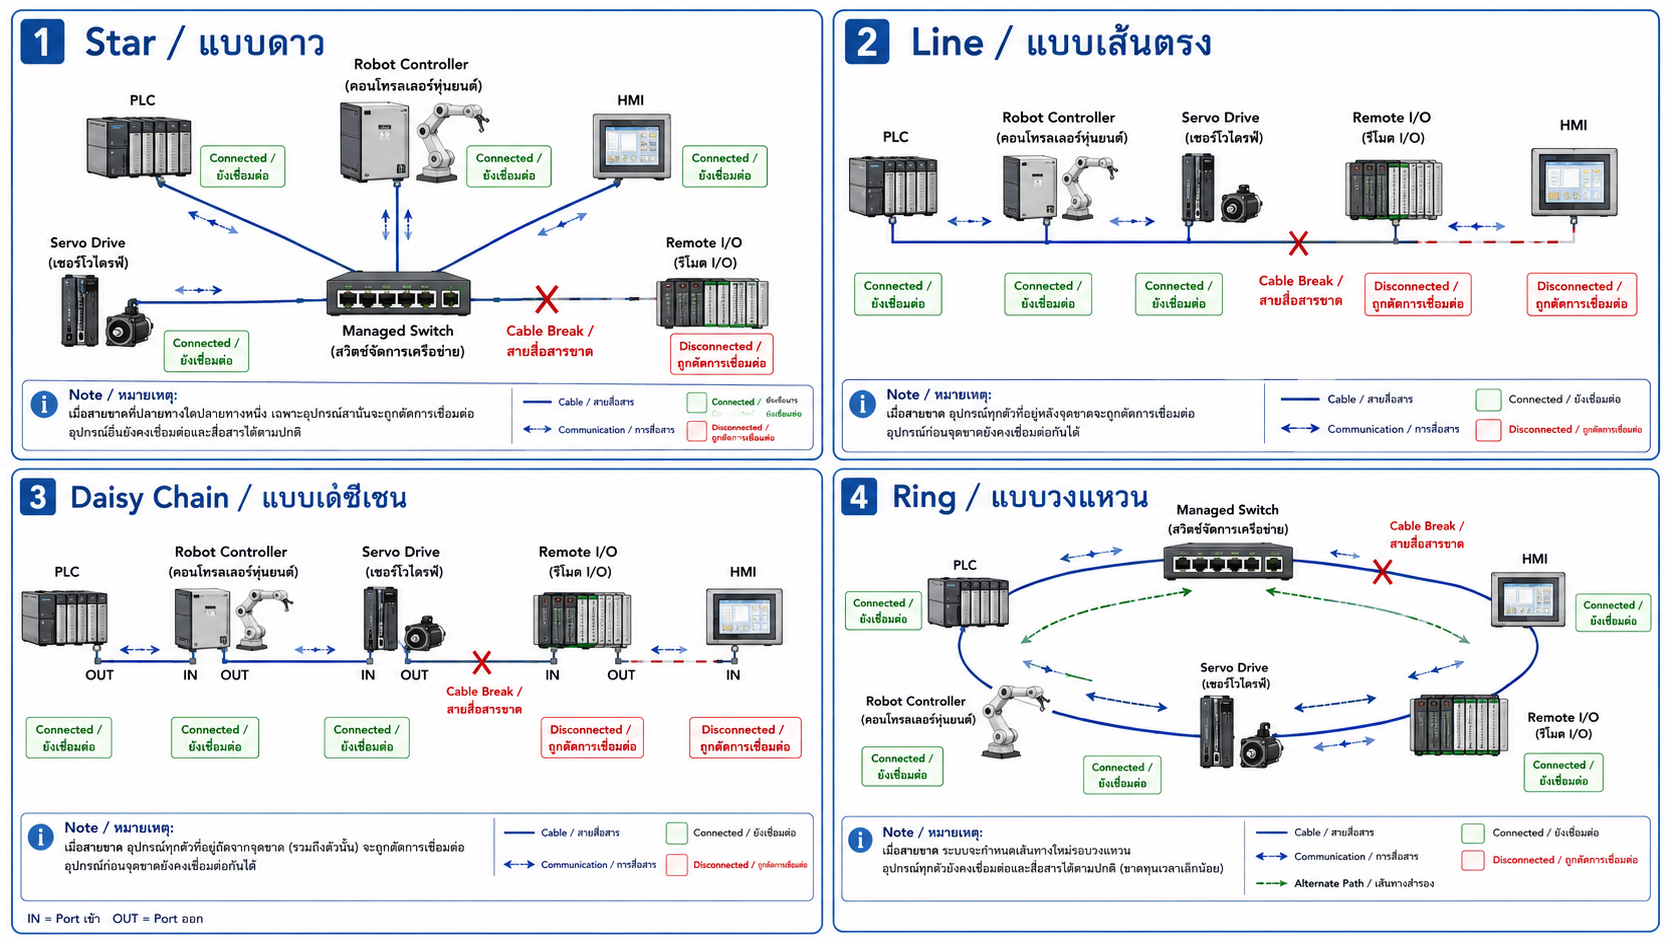
\includegraphics[width=0.8\textwidth]{images/chapter6/figure-06.png}
    \caption{โทโพโลยี Star, Line, Daisy Chain และ Ring}
\end{figure}



\subsubsection{การสื่อสารระดับสูง: OPC UA และ ROS-Industrial}

\paragraph{7.16.1 OPC UA}

OPC UA เป็นมาตรฐานที่ไม่ขึ้นกับแพลตฟอร์มสำหรับการแลกเปลี่ยนข้อมูลอย่างปลอดภัยและเชื่อถือได้ มี Information Model ที่ช่วยให้ข้อมูลมีความหมาย ไม่ใช่เพียง Address ตัวเลข จึงเหมาะกับ

\begin{itemize}
    \item Machine-to-Machine Integration
    \item เชื่อม Robot Cell กับ SCADA/MES
    \item Recipe และ Production Data
    \item Condition Monitoring
    \item Alarm และ Event
    \item Historical Data และ Digital Twin Integration
\end{itemize}

OPC UA มี Authentication, Encryption และ Integrity Mechanism แต่ต้อง Configuration Certificate, User Role และ Security Policy ให้ถูกต้อง การติดตั้งแบบเปิด Anonymous และไม่เข้ารหัสใน Production Network เพิ่มความเสี่ยง

\paragraph{7.16.2 ROS-Industrial}

ROS-Industrial ขยายความสามารถของ ROS ไปสู่งาน Manufacturing โดยมี Interface สำหรับ Industrial Manipulator, Gripper, Sensor และ Device Network รวมทั้งสนับสนุน Motion Planning, Calibration และ Perception

การใช้งานเหมาะกับงานที่ต้องการความยืดหยุ่นและ Algorithm ขั้นสูง แต่ควรแยกบทบาทจาก Safety PLC และ Servo Real-time Loop ไม่ควรถือว่า ROS Node ทั่วไปเป็น Safety-rated Controller โดยอัตโนมัติ



\subsubsection{Functional Safety กับระบบควบคุมและเครือข่าย}

Safety Function ในเซลล์หุ่นยนต์ต้องออกแบบจากการประเมินความเสี่ยงและอ้างอิงมาตรฐานที่เกี่ยวข้อง เช่น ISO 10218-1:2025 สำหรับ Industrial Robot, ISO 10218-2:2025 สำหรับ Robot Application/Cell และ IEC 60204-1 สำหรับอุปกรณ์ไฟฟ้าของเครื่องจักร

ตัวอย่าง Safety Function ได้แก่

\begin{itemize}
    \item Emergency Stop
    \item Protective Stop เมื่อประตูเปิด
    \item Safe Torque Off (STO)
    \item Safe Stop 1/2
    \item Safely Limited Speed
    \item Safe Position/Space Monitoring
    \item Enabling Device ใน Teaching Mode
\end{itemize}

\paragraph{7.17.1 Standard Control ไม่เท่ากับ Safety Control}

สัญญาณ Start, Running และ Program Select สามารถใช้ Standard I/O ได้ แต่ E-Stop และ Guard Interlock ต้องใช้ Safety-rated Architecture ตาม Performance Level หรือ SIL ที่กำหนดจาก Risk Assessment

\paragraph{7.17.2 Safety over Network}

โปรโตคอล เช่น PROFIsafe หรือ CIP Safety ส่ง Safety Data ผ่านเครือข่ายมาตรฐานด้วยกลไกตรวจสอบ เช่น Sequence, Time Expectation, Identifier และ CRC อย่างไรก็ตาม การใช้ชื่อ “Safety Protocol” ไม่เพียงพอ อุปกรณ์ทุกส่วน Configuration และ Validation ต้องรองรับระดับ Safety ที่ต้องการ

\paragraph{7.17.3 หลัก Fail-safe}

เมื่อเกิด Network Loss, Cable Break, Watchdog Timeout หรือข้อมูลไม่ถูกต้อง ระบบต้องเข้าสู่สถานะที่กำหนดไว้ล่วงหน้า โดยสถานะนั้นต้องลดความเสี่ยง ไม่ใช่เพียงหยุด Software Task



\subsubsection{การวินิจฉัยและการบำรุงรักษาเครือข่าย}

แนวทางวินิจฉัยจากชั้นล่างขึ้นชั้นบน

\begin{enumerate}
    \item \textbf{Physical:} Power, Connector, Cable, Shield, Ground, Link LED
    \item \textbf{Data Link:} MAC Error, Port Counter, Topology, Duplicate Device
    \item \textbf{Network:} IP Address, Subnet, Routing, Duplicate IP
    \item \textbf{Transport/Connection:} TCP State, UDP Loss, Connection Timeout
    \item \textbf{Application:} I/O Size, GSD/EDS/ESI, Tag Mapping, Function Code
    \item \textbf{Control Logic:} Handshake State, Interlock, Timeout, Sequence
\end{enumerate}

ข้อมูลที่ควรบันทึก

\begin{itemize}
    \item Network Diagram และ Port Map
    \item IP/Device Name Table
    \item Firmware และ Device Description Version
    \item I/O Mapping และ Data Type
    \item Cycle/Update Time
    \item Switch Configuration
    \item Baseline Error Counter
    \item Backup Configuration
\end{itemize}



\subsubsection{การเลือกโปรโตคอลให้เหมาะกับงาน}

ควรพิจารณาอย่างน้อย 8 ประเด็น

\begin{enumerate}
    \item Ecosystem ของ PLC และ Robot ที่มีอยู่
    \item Required Cycle Time และ Jitter
    \item จำนวน Axis และปริมาณ I/O
    \item ความต้องการ Motion Synchronization
    \item Diagnostics และ Predictive Maintenance
    \item Safety Communication
    \item Topology, Cable Length และสภาพแวดล้อม
    \item ทักษะบุคลากร อะไหล่ และต้นทุนตลอดอายุระบบ
\end{enumerate}

\paragraph{ตารางตัดสินใจเบื้องต้น}

\begin{table}[htbp]
    \centering
    \small
    \begin{tabularx}{\textwidth}{@{}X L{0.28\textwidth} X@{}}
        \hline
        \textbf{สถานการณ์} & \textbf{วิธีที่เหมาะสม} & \textbf{เหตุผล} \\
        \hline
        Robot เดี่ยว ต้องการ Start/Complete ไม่เกิน 20 สัญญาณ & Hard-wired I/O & เรียบง่าย วินิจฉัยง่าย ต้นทุนต่ำ \\
        ระบบเดิมมี Remote I/O จำนวนมากและใช้ Siemens & PROFIBUS DP หรือ PROFINET ตาม Controller & รักษาความเข้ากันได้และลดความเสี่ยง Migration \\
        PLC–Robot ต้องแลกสถานะและ Diagnostic จำนวนมาก & PROFINET หรือ EtherNet/IP & Cyclic I/O และ Acyclic Diagnostic \\
        Multi-axis Motion ต้อง Synchronize ต่ำกว่า 1 ms & EtherCAT, PROFINET IRT หรือ Real-time Ethernet ที่รองรับ & Timing และ Clock Synchronization ดีกว่าเครือข่าย Polling ทั่วไป \\
        ต้องเชื่อมข้อมูล Robot Cell กับ MES/Analytics & OPC UA ร่วมกับเครือข่ายควบคุม & Information Model และ Security Service \\
        งานวิจัย Vision/Motion Planning ขั้นสูง & ROS-Industrial ร่วมกับ Controller อุตสาหกรรม & Algorithm และ Interface ยืดหยุ่น แต่แยก Safety/Servo Loop \\
        \hline
    \end{tabularx}
\end{table}



\subsection{ความเข้าใจผิดที่พบบ่อย}

\subsubsection{Stepper Motor เป็นระบบวงเปิดจึงไม่มีวันคลาดเคลื่อน}

ไม่ถูกต้อง Stepper สามารถหลุด Step เมื่อโหลดสูง ความเร่งมาก หรือ Resonance เกิดขึ้น หากต้องการยืนยันตำแหน่งจริงต้องใช้ Encoder หรือเซนเซอร์อื่น

\subsubsection{\texorpdfstring{ “เพิ่ม $K_p$ ให้สูงที่สุดจะทำให้แม่นยำที่สุด”}{8.2 เพิ่ม Kp ให้สูงที่สุดจะทำให้แม่นยำที่สุด}}

$K_p$ สูงลด Error ได้ แต่เพิ่มโอกาส Overshoot, Oscillation, Noise Amplification และ Saturation ต้องพิจารณา Stability Margin และกลไกจริง

\subsubsection{“Integral Gain แก้ทุกปัญหา Error”}

Integral ช่วยกำจัด Error คงตัว แต่เพิ่ม Phase Lag และ Windup หากโหลดหรือคำสั่งเกินขีดจำกัด อาจทำให้ Recovery ช้าและ Overshoot สูง

\subsubsection{“Derivative Gain ทำให้ระบบเร็วขึ้นเสมอ”}

Derivative เพิ่ม Damping ในหลายกรณี แต่ไวต่อ Noise และการตั้งค่า Filter หากใช้ไม่เหมาะสมอาจสร้างคำสั่งกระชาก

\subsubsection{“Torque Control เท่ากับ Force Control ที่ปลายแขนโดยตรง”}

แรงบิดมอเตอร์ต้องผ่าน Gear Ratio, Efficiency, Friction, Jacobian และ Dynamics จึงจะแปลงเป็นแรงที่ปลายแขนได้

\subsubsection{“Ethernet 1 Gbps ต้องตอบสนองเร็วกว่า Fieldbus ทุกชนิด”}

Link Speed ไม่เท่ากับ Deterministic Response ต้องพิจารณา Scheduling, Stack, Switch, Load, Cycle และ Jitter

\subsubsection{“Cycle Time ที่ระบุในโบรชัวร์ใช้ได้กับทุกระบบ”}

ค่าดังกล่าวมักเป็นเงื่อนไขเฉพาะ จำนวน Node และ Payload จำกัด ต้องตรวจ Configuration จริงและ Worst-case

\subsubsection{“E-Stop ต่อเข้าขา PLC ปกติก็เพียงพอ”}

ไม่เพียงพอสำหรับ Safety Function โดยทั่วไป ต้องใช้ Safety-rated Architecture และ Validation ตาม Risk Assessment

\subsubsection{“OPC UA หรือ ROS แทน Servo Network ได้ทั้งหมด”}

OPC UA และ ROS-Industrial เหมาะกับการบูรณาการระดับข้อมูลและ Algorithm แต่ไม่แทน Hard Real-time Servo Loop หรือ Safety Function โดยอัตโนมัติ

\subsubsection{“หาก Ping ได้ แสดงว่าระบบ I/O ใช้งานได้”}

Ping ตรวจเพียง IP Connectivity บางส่วน ไม่ยืนยัน Device Name, I/O Module, Connection, Data Mapping หรือ Application State



\subsection{การประยุกต์ใช้ในงานจริง}

\subsubsection{เซลล์ Pick and Place กับสายพาน}

PLC รับ Photoelectric Sensor ตรวจชิ้นงาน ควบคุม Conveyor และส่ง Part Ready ไป Robot เมื่อ Robot พร้อมและพื้นที่ปลอดภัย PLC ส่ง Start Request Robot เคลื่อนด้วย Position Control และใช้ Vacuum Sensor ยืนยันการจับ หากจับไม่สำเร็จ Robot ส่ง Grip Fault ให้ PLC จัดการ Reject Sequence

\subsubsection{งาน Press-fit}

Robot เคลื่อนเข้าใกล้ด้วย Position Control จากนั้นเปลี่ยนเป็น Force/Torque Control หรือ Impedance Mode ใกล้ผิวสัมผัส ใช้ Force Sensor หรือ Motor Torque Estimate ตรวจแรงกด PLC บันทึก Peak Force และ Displacement ผ่าน Industrial Ethernet เพื่อประเมินคุณภาพ

\subsubsection{งานเชื่อมแบบหลายสถานี}

PLC ควบคุม Fixture, Fume Extraction และ Safety Interlock หุ่นยนต์รับ Program Number ตามรุ่นชิ้นงาน PROFINET หรือ EtherNet/IP ส่งสถานะ Welding, Arc Fault และ Cycle Complete ข้อมูล Production Count ส่งต่อ OPC UA ไป MES

\subsubsection{ระบบ Multi-axis Packaging}

Servo หลายแกนต้อง Synchronize กับ Conveyor Encoder จึงใช้ Real-time Ethernet ที่มี Distributed Clock หรือ Isochronous Mode วงรอบ Motion ทำงานระดับ Controller ส่วน PLC Sequence จัดการ Recipe และ Alarm

\subsubsection{Condition Monitoring}

Servo Drive ส่งข้อมูล Current, Torque, Temperature และ Following Error ผ่าน Acyclic Diagnostic ระบบวิเคราะห์แนวโน้มเพื่อระบุ Gear Wear, Bearing Friction หรือ Load Change โดยไม่แทรกแซงวงรอบควบคุมหลัก



\subsection{สรุปท้ายบท}

\begin{enumerate}
    \item ระบบวงเปิดไม่มี Feedback จึงง่ายและต้นทุนต่ำ แต่ไม่ชดเชยความคลาดเคลื่อนจากโหลดและ Disturbance โดยตรง
    \item ระบบวงปิดคำนวณ Error จากค่าตั้งและค่าที่วัด จึงเพิ่มความแม่นยำได้ แต่ต้องออกแบบเสถียรภาพ Bandwidth และ Noise Sensitivity
    \item PID ประกอบด้วยพจน์ P, I และ D ซึ่งมีบทบาทต่างกัน การปรับ Gain ต้องประเมิน Rise Time, Overshoot, Settling Time, Steady-state Error และ Control Effort
    \item Servo Axis มักใช้วงรอบซ้อน Current–Speed–Position โดยวงด้านในต้องเร็วกว่าและคงตัวก่อนวงด้านนอก
    \item Joint Space Control เหมาะกับการควบคุมตัวแปรข้อต่อ ส่วน Cartesian Space Control เหมาะกับเส้นทางและแรงที่ End Effector แต่ต้องใช้ Kinematics และ Jacobian
    \item Computed Torque Control ใช้แบบจำลอง Dynamics ชดเชย Inertia, Coriolis และ Gravity แต่ไวต่อ Model Error
    \item PLC และ Robot Controller ควรแลกคำสั่งด้วย Handshake, Interlock และ Timeout ไม่พึ่ง Pulse เดี่ยวโดยไม่มีการยืนยัน
    \item Standard I/O ต้องแยกจาก Safety-rated I/O โดยเฉพาะ E-Stop และ Guard Door
    \item การเลือก Fieldbus หรือ Industrial Ethernet ต้องพิจารณา Determinism, Cycle Time, Jitter, Diagnostics, Topology และ Ecosystem ไม่พิจารณา Link Speed เพียงอย่างเดียว
    \item PROFINET, EtherNet/IP, EtherCAT, Modbus TCP และ POWERLINK มีจุดเด่นต่างกัน ค่าประสิทธิภาพจริงขึ้นกับอุปกรณ์ Configuration และ Network Load
    \item OPC UA และ ROS-Industrial ช่วยบูรณาการระดับข้อมูลและ Algorithm แต่ไม่แทนวงรอบ Servo และ Functional Safety โดยอัตโนมัติ
    \item การวินิจฉัยควรเริ่มจาก Physical Layer ไปยัง Application และ Control Logic พร้อมเอกสาร Network Baseline ที่ครบถ้วน
\end{enumerate}



\subsection{คำถามทบทวนท้ายบท}

\begin{enumerate}
    \item อธิบายความแตกต่างระหว่าง Open-loop Control และ Closed-loop Control พร้อมยกตัวอย่างจากระบบหุ่นยนต์อย่างละหนึ่งตัวอย่าง
    \item เหตุใดการเพิ่ม $K_p$ มากเกินไปจึงอาจทำให้ระบบสั่น แม้ Steady-state Error จะลดลง
    \item Integral Windup เกิดขึ้นได้อย่างไร และมีแนวทางป้องกันอย่างไร
    \item เปรียบเทียบ Position, Speed และ Torque Control ในด้านตัวแปรป้อนกลับ งานที่เหมาะสม และข้อจำกัด
    \item เพราะเหตุใด Current Loop จึงต้องเร็วกว่าวงรอบ Speed และ Position
    \item Joint Space Control และ Cartesian Space Control แตกต่างกันอย่างไร และงานเชื่อมแนวเส้นตรงควรให้ความสำคัญกับวิธีใด
    \item อธิบายบทบาทของ Jacobian Matrix ในการควบคุมหุ่นยนต์
    \item เหตุใด PLC–Robot Interface จึงควรใช้ Handshake และ Timeout แทน Start Pulse เพียงสัญญาณเดียว
    \item เปรียบเทียบ Hard-wired I/O, Fieldbus และ Industrial Ethernet ในด้านปริมาณข้อมูล การวินิจฉัย และความซับซ้อน
    \item Modbus RTU และ Modbus TCP เหมือนและต่างกันอย่างไร
    \item เหตุใด EtherCAT จึงเหมาะกับงาน Multi-axis Motion มากกว่า Modbus TCP ในหลายกรณี
    \item Cycle Time, Latency และ Jitter แตกต่างกันอย่างไร
    \item Star, Line และ Ring Topology มีผลต่อความทนทานเมื่อสายขาดอย่างไร
    \item เหตุใด Emergency Stop จึงไม่ควรพึ่ง Standard PLC I/O เพียงอย่างเดียว
    \item OPC UA และ ROS-Industrial ควรอยู่ในระดับใดของสถาปัตยกรรม และเหตุใดจึงไม่ควรแทน Servo Loop โดยตรง
\end{enumerate}

\newpage

\subsection{กิจกรรมปฏิบัติการประจำบท}

\subsubsection{กิจกรรมปฏิบัติการที่ 6-1: การตั้งค่า PID และวิเคราะห์ Step Response ของ Servo Axis}

\paragraph{1. วัตถุประสงค์}

หลังปฏิบัติ นักศึกษาสามารถ

\begin{enumerate}
    \item ตั้งค่าการทดลอง Servo Axis ในโหมดที่ผู้ผลิตอนุญาตภายใต้ขีดจำกัดปลอดภัย
    \item ปรับค่า $K_p$, $K_i$ และ $K_d$ หรือค่าพารามิเตอร์เทียบเท่าของ Drive อย่างเป็นระบบ
    \item วัด Rise Time, Overshoot, Settling Time และ Steady-state Error
    \item วิเคราะห์ Trade-off ระหว่างความเร็ว ความแม่นยำ การสั่น และ Control Effort
    \item เลือกชุด Gain ที่เหมาะสมตามเกณฑ์ที่กำหนด
\end{enumerate}

\paragraph{2. หลักการและทฤษฎีที่เกี่ยวข้อง}

ใช้หลักการ PID ในหัวข้อ 7.4 และตัวชี้วัด Step Response ในหัวข้อ 7.3 การทดลองไม่มุ่งหาค่า Gain สูงสุด แต่หาค่าที่ทำให้ระบบผ่านเกณฑ์หลายด้านพร้อมกัน

ตัวชี้วัดหลัก

\[
M_p(\%)=\frac{y_{max}-y_{ss}}{y_{ss}}\times100
\]

และกำหนด Settling Time จากช่วงที่ผลตอบสนองอยู่ภายในแถบ $\pm2\%$ ของค่าปลายทาง หรือเกณฑ์ที่ผู้สอนกำหนด

\paragraph{3. อุปกรณ์ เครื่องมือ และซอฟต์แวร์}

\begin{enumerate}
    \item ชุดทดลอง Servo Drive และ Servo Motor แบบการศึกษา ชนิดติดตั้งสำเร็จ มี Guard ครอบเพลา จำนวน 1 ชุดต่อกลุ่ม
    \item แหล่งจ่ายและตู้ควบคุมที่ผู้ผลิตจัดให้ พร้อม Protective Earth
    \item Encoder ที่ติดมากับ Servo Motor
    \item โหลดปรับได้แบบมี Guard และค่าพิกัดไม่เกินคู่มือ
    \item Oscilloscope แบบ Isolated Input หรือ Data Acquisition ที่ผู้ผลิตอนุญาต
    \item คอมพิวเตอร์และซอฟต์แวร์ Commissioning ของ Servo Drive
    \item Emergency Stop และ Main Isolator ที่ผ่านการตรวจสอบก่อนเรียน
    \item แบบบันทึกผลและไฟล์ Configuration สำรอง
\end{enumerate}

\begin{quote}
หากไม่มี Servo Trainer จริง ให้ใช้ Digital Twin หรือ Simulator ของผู้ผลิตเพื่อศึกษาผลของ Gain โดยไม่สั่งมอเตอร์จริง
\end{quote}

\paragraph{4. แผนภาพชุดทดลอง}

\begin{verbatim}
PC Commissioning Software
          |
          v
Educational Servo Drive -- Current/Speed/Position Data --> Oscilloscope/Logger
          |
          v
Guarded Servo Motor -- Guarded Coupling -- Adjustable Educational Load
          ^
          | Encoder Feedback

Safety Chain: E-Stop -> Safety Relay/STO -> Servo Drive
\end{verbatim}

\paragraph{5. ข้อควรระวังด้านความปลอดภัย}

\begin{enumerate}
    \item ปฏิบัติภายใต้การกำกับของผู้สอนหรือผู้รับผิดชอบห้องปฏิบัติการ
    \item ใช้ชุดทดลองที่มี Guard ครอบเพลาและชิ้นส่วนหมุน ห้ามถอด Guard ขณะจ่ายพลังงาน
    \item ตรวจ E-Stop, STO และ Main Isolator ก่อนเริ่มทุกครั้ง
    \item ห้ามต่อ Probe เข้าวงจร Power Stage โดยตรง ใช้เฉพาะ Monitoring Port หรือ Isolated Measurement ที่ผู้ผลิตกำหนด
    \item จำกัด Speed, Torque, Travel และ Acceleration ให้อยู่ในค่าที่ผู้สอนกำหนด
    \item ห้ามปรับ Gain แบบก้าวกระโดดหรือปิด Protection Function
    \item หากได้ยินเสียงผิดปกติ เกิดการสั่นต่อเนื่อง หรือมี Alarm ให้กด Stop/E-Stop ตามขั้นตอนและแจ้งผู้สอน
    \item ห้ามจับเพลา Coupling หรือโหลดจนกว่าจะตัดพลังงานและยืนยันว่าไม่มีพลังงานสะสม
\end{enumerate}

\paragraph{6. ขั้นตอนการปฏิบัติ}

\textbf{ตอนที่ A ตรวจสอบระบบ}

\begin{enumerate}
    \item ตัดพลังงานและตรวจการต่อสายกับแผนภาพของผู้ผลิต
    \item ตรวจ Guard, Protective Earth และ Emergency Stop
    \item เปิดซอฟต์แวร์และบันทึกค่าพารามิเตอร์เดิมเป็น Backup
    \item กำหนด Current/Torque Limit, Speed Limit และ Acceleration Limit ตามใบงาน
    \item ทดสอบ Jog ที่ความเร็วต่ำเพื่อยืนยัน Encoder Direction และ Motor Direction
\end{enumerate}

\textbf{ตอนที่ B เก็บ Baseline}

\begin{enumerate}
    \item ใช้ค่า Gain มาตรฐานจากผู้ผลิตหรือค่าที่ผู้สอนจัดเตรียม
    \item สั่ง Step หรือ Speed Change ขนาดเล็กตามที่ชุดทดลองรองรับ
    \item บันทึก Command, Actual, Error และ Control Output
    \item ทำซ้ำอย่างน้อย 3 ครั้งและตรวจความสม่ำเสมอ
\end{enumerate}

\textbf{ตอนที่ C ปรับ $K_p$}

\begin{enumerate}
    \item กำหนด $K_i=0$ และ $K_d=0$ หาก Controller อนุญาตและผู้สอนกำหนด
    \item เพิ่ม $K_p$ ทีละขั้นขนาดเล็ก
    \item บันทึก Rise Time, Overshoot, Settling Time, Error และอาการสั่น
    \item หยุดเพิ่มเมื่อถึงขีดจำกัดที่ผู้สอนกำหนดหรือเริ่มเห็นแนวโน้มสั่น
\end{enumerate}

\textbf{ตอนที่ D ปรับ $K_i$}

\begin{enumerate}
    \item เลือก $K_p$ ที่ตอบสนองดีแต่ยังมี Margin
    \item เพิ่ม $K_i$ ทีละขั้นเพื่อแก้ Steady-state Error
    \item ทดสอบ Saturation ด้วยคำสั่งที่ยังอยู่ในขีดจำกัด และสังเกต Windup โดยไม่เกินค่าปลอดภัย
    \item เปิดใช้ Anti-windup หาก Drive รองรับ แล้วเปรียบเทียบ Recovery
\end{enumerate}

\textbf{ตอนที่ E ปรับ $K_d$ หรือ Damping Parameter}

\begin{enumerate}
    \item เพิ่มค่าอนุพันธ์หรือ Damping ทีละน้อย
    \item ตรวจ Noise ที่ Control Output และสังเกตผลของ Filter
    \item เลือกชุด Gain สุดท้ายตามเกณฑ์ เช่น Overshoot < 5\%, Settling Time < ค่าที่กำหนด และไม่มีการสั่นต่อเนื่อง
\end{enumerate}

\paragraph{7. ตารางบันทึกผล}

\begin{table}[htbp]
    \centering
    \resizebox{\textwidth}{!}{%
    \begin{tabular}{r r r r r r r r r l l}
        \hline
        \textbf{ชุดทดลอง} & \textbf{$K_p$} & \textbf{$K_i$} & \textbf{$K_d$} & \textbf{Rise Time (s)} & \textbf{Overshoot (\%)} & \textbf{Settling Time (s)} & \textbf{$e_{ss}$} & \textbf{Peak Output} & \textbf{อาการสั่น/Noise} & \textbf{ผ่านเกณฑ์} \\
        \hline
        Baseline &  &  &  &  &  &  &  &  &  &  \\
        P-1 &  & 0 & 0 &  &  &  &  &  &  &  \\
        P-2 &  & 0 & 0 &  &  &  &  &  &  &  \\
        PI-1 &  &  & 0 &  &  &  &  &  &  &  \\
        PID-1 &  &  &  &  &  &  &  &  &  &  \\
        Final &  &  &  &  &  &  &  &  &  &  \\
        \hline
    \end{tabular}
    }
\end{table}

\paragraph{8. การคำนวณและวิเคราะห์ผล}

\begin{enumerate}
    \item คำนวณ Overshoot จากข้อมูลที่วัด
    \item ระบุเกณฑ์ Rise Time และ Settling Band ที่ใช้
    \item สร้างกราฟเปรียบเทียบอย่างน้อย 3 ชุด Gain
    \item วิเคราะห์ว่าการเพิ่ม Gain แต่ละพจน์เปลี่ยน Control Effort อย่างไร
    \item ตรวจว่าชุด Gain ที่เร็วที่สุดเป็นชุดที่เหมาะสมที่สุดหรือไม่
    \item อภิปรายความแตกต่างระหว่างผลจริงกับแนวโน้มในตารางทฤษฎี
\end{enumerate}

\paragraph{9. การเปรียบเทียบผลจริงกับทฤษฎี}

ผลจริงอาจไม่ตรงแนวโน้มทั่วไปเนื่องจาก

\begin{itemize}
    \item Drive ใช้ PID Form หรือ Gain Scaling ต่างจากสมการมาตรฐาน
    \item มี Feedforward, Filter, Notch Filter หรือ Auto-tuning ทำงานอยู่
    \item Plant มี Backlash, Friction และ Resonance
    \item Sampling Time และ Data Logging Rate จำกัด
    \item Output Saturation และ Anti-windup เปลี่ยนพฤติกรรม
\end{itemize}

\paragraph{10. คำถามหลังการทดลอง}

\begin{enumerate}
    \item ชุด Gain ใดให้ Rise Time ต่ำที่สุด และมีข้อเสียใด
    \item $K_i$ ช่วยลด Error ได้จริงหรือไม่ และทำให้ Overshoot เปลี่ยนอย่างไร
    \item เมื่อเกิด Saturation ระบบใช้เวลาฟื้นตัวเท่าใดก่อนและหลัง Anti-windup
    \item $K_d$ หรือ Damping Parameter เพิ่ม Noise หรือไม่
    \item หากเพิ่มโหลด ผลตอบสนองและค่า Gain ที่เหมาะสมเปลี่ยนอย่างไร
\end{enumerate}

\paragraph{11. เกณฑ์การประเมิน}

\begin{table}[htbp]
    \centering
    \begin{tabular}{l r}
        \hline
        \textbf{ด้านที่ประเมิน} & \textbf{คะแนน} \\
        \hline
        ตรวจสอบความปลอดภัยและปฏิบัติตามขั้นตอน & 20 \\
        การตั้งค่าและเก็บข้อมูลถูกต้อง & 20 \\
        การคำนวณตัวชี้วัด & 20 \\
        การวิเคราะห์ Trade-off และเลือก Gain & 25 \\
        รายงาน กราฟ และการอภิปราย & 15 \\
        \textbf{รวม} & \textbf{100} \\
        \hline
    \end{tabular}
\end{table}



\subsubsection{กิจกรรมปฏิบัติการที่ 6-2: การเชื่อมต่อ PLC กับ Robot Controller ผ่าน Hard-wired I/O}

\paragraph{1. วัตถุประสงค์}

หลังปฏิบัติ นักศึกษาสามารถ

\begin{enumerate}
    \item จัดทำ I/O List และ Wiring Diagram สำหรับ PLC–Robot Interface
    \item ต่อ Standard 24 VDC I/O เมื่อระบบถูกตัดพลังงานและตรวจสอบแล้ว
    \item เขียน Ladder Logic สำหรับ Handshake, Interlock และ Timeout
    \item ทดสอบ Start, Running, Complete, Fault และ Reset Sequence
    \item อธิบายการแยก Standard Control จาก Safety Circuit ได้
\end{enumerate}

\paragraph{2. หลักการและทฤษฎีที่เกี่ยวข้อง}

ใช้แนวคิด Digital I/O, PNP/NPN, Handshake, Program Select และ Timeout ในหัวข้อ 7.8 โดยกำหนด State Machine อย่างน้อย 5 สถานะ

\begin{verbatim}
IDLE -> REQUEST -> ACKNOWLEDGED -> RUNNING -> COMPLETE -> IDLE
                      +------------ FAULT ------------+
\end{verbatim}

\paragraph{3. อุปกรณ์ เครื่องมือ และซอฟต์แวร์}

\begin{enumerate}
    \item PLC Trainer 24 VDC จำนวน 1 ชุด
    \item Robot Controller Simulator หรือ Educational Robot Cell ที่มี Standard I/O Interface
    \item Interface Relay/Optocoupler Module ตามชนิด I/O
    \item Terminal Block, Fuse และสาย Patch สำหรับการศึกษา
    \item Multimeter CAT-rated ที่เหมาะสมกับ 24 VDC
    \item คอมพิวเตอร์และ PLC Programming Software
    \item Safety Relay/Guard Circuit ที่ \textbf{ติดตั้งและตรวจสอบล่วงหน้าโดยผู้สอน}
    \item Emergency Stop และ Guard ที่เป็นส่วนหนึ่งของชุดฝึก
\end{enumerate}

\paragraph{4. แผนภาพหรือวงจร}

Standard I/O ที่ใช้ในการทดลอง

\begin{table}[htbp]
    \centering
    \begin{tabular}{l l l}
        \hline
        \textbf{PLC Output \(\to\) Robot Input} & \textbf{PLC Address} & \textbf{Robot Signal} \\
        \hline
        Start\_Request & Q0.0 & DI\_START\_REQ \\
        Reset\_Request & Q0.1 & DI\_RESET\_REQ \\
        Program\_Bit0 & Q0.2 & DI\_PROG\_0 \\
        Program\_Bit1 & Q0.3 & DI\_PROG\_1 \\
        Program\_Bit2 & Q0.4 & DI\_PROG\_2 \\
        Program\_Bit3 & Q0.5 & DI\_PROG\_3 \\
        \hline
    \end{tabular}
\end{table}

\begin{table}[htbp]
    \centering
    \begin{tabular}{l l l}
        \hline
        \textbf{Robot Output \(\to\) PLC Input} & \textbf{Robot Signal} & \textbf{PLC Address} \\
        \hline
        Ready & DO\_READY & I0.0 \\
        Start\_Ack & DO\_START\_ACK & I0.1 \\
        Running & DO\_RUNNING & I0.2 \\
        Complete & DO\_COMPLETE & I0.3 \\
        Fault & DO\_FAULT & I0.4 \\
        Home & DO\_HOME & I0.5 \\
        \hline
    \end{tabular}
\end{table}

\paragraph{5. ข้อควรระวังด้านความปลอดภัย}

\begin{enumerate}
    \item การต่อสายทำเฉพาะวงจร 24 VDC Standard I/O และต้องตัดพลังงานก่อนทุกครั้ง
    \item Safety Circuit ต้องติดตั้งล่วงหน้าโดยผู้มีอำนาจและห้ามนักศึกษาดัดแปลง
    \item E-Stop ใช้ Safety Relay/Safety PLC ไปยัง Robot Safety Interface ไม่ผ่าน Standard PLC Output
    \item ทดสอบ Logic ใน Simulator ก่อนอนุญาต Motion จริง
    \item หากใช้ Robot จริง ให้จำกัดความเร็วและพื้นที่ พร้อมผู้สอนควบคุม Pendant
    \item ตรวจ PNP/NPN และ Common 0 V ก่อนจ่ายไฟ
    \item ใช้ Fuse แยก Branch และห้าม Short Terminal เพื่อจำลอง Fault
    \item การจำลอง Fault ใช้ Software Flag หรือ Disconnect Plug ที่ออกแบบสำหรับ Trainer เท่านั้น
\end{enumerate}

\paragraph{6. ขั้นตอนการปฏิบัติ}

\textbf{ตอนที่ A ออกแบบ}

\begin{enumerate}
    \item จัดทำ I/O List และกำหนดทิศทางสัญญาณ
    \item วาด Wiring Diagram แยก Standard I/O กับ Safety Circuit
    \item กำหนด State Machine และ Timeout ของแต่ละขั้น
    \item ตรวจแบบร่วมกับผู้สอน
\end{enumerate}

\textbf{ตอนที่ B ต่อวงจร Standard I/O}

\begin{enumerate}
    \item ตัดพลังงานและ Lock/Tag ตามขั้นตอนห้องปฏิบัติการ
    \item ต่อ PLC Output ผ่าน Interface Module ไป Robot Input
    \item ต่อ Robot Output กลับ PLC Input
    \item ตรวจ Continuity และขั้ว Common
    \item ให้ผู้สอนตรวจและอนุญาตก่อนจ่าย 24 VDC
\end{enumerate}

\textbf{ตอนที่ C เขียน Ladder Logic}

\begin{enumerate}
    \item สร้าง Permissive: Ready AND Home AND No Fault AND Cell Safe Status
    \item Latch Cycle Request เมื่อกด Start และ Permissive ครบ
    \item ส่ง Start\_Request จนได้รับ Start\_Ack
    \item เริ่ม Timer หาก Ack ไม่มาภายในเวลาที่กำหนด
    \item เมื่อ Running เป็น 1 ให้เข้าสถานะ RUNNING
    \item เมื่อ Complete เป็น 1 ให้บันทึก Cycle Complete และ Reset Request ตาม Handshake
    \item เมื่อ Fault เป็น 1 ให้ยกเลิกคำสั่ง Start และเข้าสถานะ FAULT
\end{enumerate}

\textbf{ตอนที่ D ทดสอบ}

\begin{enumerate}
    \item ทดสอบ Normal Cycle อย่างน้อย 3 รอบ
    \item ทดสอบ Robot Not Ready
    \item ทดสอบ Start\_Ack Timeout ผ่าน Simulator
    \item ทดสอบ Fault ระหว่าง Running
    \item ทดสอบการคืนระบบหลัง Reset ตามคู่มือ
    \item ให้ผู้สอนสาธิตการทำงานของ Safety Circuit แยกจาก Standard Logic โดยไม่ให้นักศึกษาปรับแก้
\end{enumerate}

\paragraph{7. ตารางบันทึกผล}

\begin{table}[htbp]
    \centering
    \resizebox{\textwidth}{!}{%
    \begin{tabular}{l r r r r r r r r l l}
        \hline
        \textbf{Test Case} & \textbf{Ready} & \textbf{Home} & \textbf{Fault} & \textbf{Start Req} & \textbf{Start Ack} & \textbf{Running} & \textbf{Complete} & \textbf{Timeout} & \textbf{ผลที่คาดหวัง} & \textbf{ผลที่สังเกต} \\
        \hline
        Normal cycle & 1 & 1 & 0 & 1 & 1 & 1 & 1 & 0 & จบรอบปกติ &  \\
        Not ready & 0 & 1 & 0 & 0 & 0 & 0 & 0 & 0 & ไม่ส่ง Start &  \\
        Ack timeout & 1 & 1 & 0 & 1 & 0 & 0 & 0 & 1 & เข้าสถานะ Fault &  \\
        Fault during run & 1 & 1 & 1 & 0 & - & 0 & 0 & - & ยกเลิก Sequence &  \\
        Reset recovery & 1 & 1 & 0 & 0 & 0 & 0 & 0 & 0 & กลับ IDLE &  \\
        \hline
    \end{tabular}
    }
\end{table}

\paragraph{8. การคำนวณและวิเคราะห์ผล}

\begin{enumerate}
    \item วัดเวลาจาก Start\_Request ถึง Running
    \item วัดเวลาจาก Complete ถึง PLC รับรู้
    \item เปรียบเทียบกับ PLC Scan และ Input Filter
    \item ประเมิน Timeout ที่เหมาะสมโดยมี Margin
    \item ตรวจว่าคำสั่ง Start ถูกยกเลิกเมื่อ Fault หรือ Permissive หายหรือไม่
\end{enumerate}

\paragraph{9. การเปรียบเทียบผลจริงกับทฤษฎี}

ความล่าช้าอาจเกิดจาก Input Filter, PLC Scan, Relay Delay, Robot Task และ Debounce การใช้ Relay เพิ่ม Isolation แต่เพิ่ม Delay และจุดสึกหรอ จึงควรเลือกตามความต้องการและจำนวนรอบ

\paragraph{10. คำถามหลังการทดลอง}

\begin{enumerate}
    \item หาก Start\_Request เป็น Pulse สั้นกว่า PLC/Robot Scan จะเกิดปัญหาใด
    \item เหตุใด Start\_Ack ต้องตอบกลับก่อน PLC ปิด Request
    \item Timeout สั้นและยาวเกินไปมีผลอย่างไร
    \item ถ้า Robot Fault ระหว่าง Running PLC ควรเก็บสถานะใดไว้เพื่อวินิจฉัย
    \item Safety Circuit แตกต่างจาก Standard Interlock ในด้านใด
\end{enumerate}

\paragraph{11. เกณฑ์การประเมิน}

\begin{table}[htbp]
    \centering
    \begin{tabular}{l r}
        \hline
        \textbf{ด้านที่ประเมิน} & \textbf{คะแนน} \\
        \hline
        I/O List และ Wiring Diagram & 20 \\
        การต่อวงจร 24 VDC อย่างปลอดภัย & 20 \\
        Ladder Handshake และ Timeout & 25 \\
        การทดสอบกรณีปกติและ Fault & 20 \\
        การวิเคราะห์และรายงาน & 15 \\
        \textbf{รวม} & \textbf{100} \\
        \hline
    \end{tabular}
\end{table}

\newpage

\subsection{แบบฝึกหัดท้ายบท}

\subsubsection{ระดับพื้นฐาน}

\textbf{ข้อ 1} \\
อธิบายความหมายของ Setpoint, Actual Value และ Error ในระบบควบคุมตำแหน่งของข้อต่อหุ่นยนต์

\textbf{ข้อ 2} \\
ระบุข้อดีสองข้อและข้อจำกัดสองข้อของระบบควบคุมวงเปิด

\textbf{ข้อ 3} \\
ตัวควบคุม PID มี $K_p=3$, $K_i=0.5\ \text{s}^{-1}$ และ $K_d=0.2\ \text{s}$ ณ ขณะหนึ่ง $e=0.4$, $\int e\,dt=0.6$ และ $de/dt=-0.5$ จงคำนวณ $u$

\textbf{ข้อ 4} \\
ระบบตำแหน่งได้รับคำสั่ง $50^\circ$ และมีค่าสูงสุด $57^\circ$ ก่อนคงตัวที่ $50^\circ$ จงคำนวณ Overshoot เป็นร้อยละ

\textbf{ข้อ 5} \\
เปรียบเทียบข้อมูล Cyclic และ Acyclic พร้อมยกตัวอย่างอย่างละสองรายการใน Robot–PLC Network

\subsubsection{ระดับวิเคราะห์}

\textbf{ข้อ 6} \\
ระบบ Servo มี Current Loop Bandwidth 1500 Hz หากใช้อัตราส่วนเริ่มต้น 5:1 ระหว่างวงรอบ จงประมาณ Speed Loop และ Position Loop Bandwidth พร้อมอธิบายเหตุผลที่ต้องแยก Bandwidth

\textbf{ข้อ 7} \\
ระบบ Joint Position Control มี Plant Gain $G=1.2$ และใช้ Proportional Controller $K_p=5$ กับ Unity Feedback จงหา Closed-loop Static Gain และ Steady-state Error เมื่อสั่ง Step ขนาด 1 หน่วย

\textbf{ข้อ 8} \\
Torque Sensor ช่วง 4–20 mA แทนแรงบิด $-100$ ถึง $300\ \text{N·m}$ หากวัดได้ 10 mA จงคำนวณแรงบิด

\textbf{ข้อ 9} \\
PLC Scan 10 ms, Input Filter 3 ms, Network Update ไปและกลับด้านละ 2 ms, Robot Processing 15 ms และ Output Delay 4 ms จงประมาณเวลาตอบสนองรวม พร้อมเสนอ Timeout ขั้นต่ำที่สมเหตุสมผลสำหรับ Handshake ที่ไม่ใช่ Safety

\textbf{ข้อ 10} \\
โรงงานมี Robot 1 ตัว ต้องการเพียง Start, Reset, Ready, Running, Complete, Fault และ Program Select 4 บิต ระยะสาย 15 m ไม่มีความต้องการ Diagnostic จำนวนมาก จงเปรียบเทียบ Hard-wired I/O กับ Industrial Ethernet และเสนอวิธีที่เหมาะสม

\subsubsection{13.3 ระดับประยุกต์ใช้}

\textbf{ข้อ 11} \\
ออกแบบ I/O Handshake สำหรับเซลล์ Pick and Place ที่มี PLC, Robot, Conveyor และ Gripper โดยระบุอย่างน้อย 6 สัญญาณจาก PLC ไป Robot, 6 สัญญาณจาก Robot ไป PLC, ลำดับ Normal Cycle และ Timeout/Fault Handling

\textbf{ข้อ 12} \\
สายการผลิตต้องควบคุม Servo 12 แกนให้ Synchronize ด้วย Cycle Time ต่ำกว่า 1 ms พร้อมอ่าน Remote I/O และส่งข้อมูล Production ไป MES จงเสนอ Architecture ที่แยก Motion Network, PLC/Cell Network และ Information Network พร้อมเหตุผล

\textbf{ข้อ 13} \\
ระหว่างทดสอบ PROFINET ระหว่าง S7-1500 กับ Robot พบว่า Link LED ติดและ Ping ได้ แต่ PLC แสดง Device Not Reachable และไม่มี I/O Data จงสร้างลำดับวินิจฉัยอย่างน้อย 8 ขั้นตอน โดยเริ่มจาก Physical/Identification ไปยัง Configuration และ Application Mapping

\newpage

\subsection{แนวคำตอบแบบฝึกหัดสำหรับผู้สอน}

\subsubsection{14.1 ระดับพื้นฐาน}

\textbf{แนวคำตอบข้อ 1} \\
Setpoint คือตำแหน่งที่ต้องการ เช่น $30^\circ$; Actual Value คือตำแหน่งที่ Encoder วัดได้; Error คือผลต่าง $e=q_d-q$ หาก Setpoint $30^\circ$ และวัดได้ $28^\circ$ จะมี Error $2^\circ$

\textbf{แนวคำตอบข้อ 2} \\
ข้อดี เช่น โครงสร้างง่าย ต้นทุนต่ำ และไม่ต้องใช้เซนเซอร์บางกรณี ข้อจำกัด เช่น ไม่ทราบความคลาดเคลื่อนจริงและไม่ชดเชยโหลดเปลี่ยนโดยตรง

\textbf{แนวคำตอบข้อ 3}

\[
u=K_pe+K_i\int e\,dt+K_d\frac{de}{dt}
\]

\[
u=3(0.4)+0.5(0.6)+0.2(-0.5)
\]

\[
u=1.2+0.3-0.1=1.4
\]

ดังนั้น $u=1.4$ หน่วยคำสั่ง

\textbf{แนวคำตอบข้อ 4}

\[
M_p=\frac{57-50}{50}\times100=14\%
\]

\textbf{แนวคำตอบข้อ 5} \\
Cyclic Data ส่งเป็นรอบ เช่น Ready, Running, Actual Position และ I/O Process Data ส่วน Acyclic Data ส่งเมื่อร้องขอ เช่น Parameter, Device Identification, Alarm History และ Diagnostic Record

\subsubsection{14.2 ระดับวิเคราะห์}

\textbf{แนวคำตอบข้อ 6}

\[
f_v=\frac{1500}{5}=300\ \text{Hz}
\]

\[
f_p=\frac{300}{5}=60\ \text{Hz}
\]

ต้องแยก Bandwidth เพื่อให้วงด้านในเข้าสู่สภาวะตอบสนองก่อนวงด้านนอก ลดการรบกวนกันและทำให้การออกแบบแต่ละวงง่ายขึ้น ค่าจริงต้องยืนยันกับ Plant

\textbf{แนวคำตอบข้อ 7}

\[
T=\frac{K_pG}{1+K_pG}=\frac{5(1.2)}{1+5(1.2)}=\frac{6}{7}=0.8571
\]

สำหรับ Step ขนาด 1

\[
e_{ss}=1-0.8571=0.1429
\]

หรือประมาณ 14.29\%

\textbf{แนวคำตอบข้อ 8}

\[
\tau=-100+\frac{10-4}{16}[300-(-100)]
\]

\[
\tau=-100+\frac{6}{16}(400)=-100+150=50\ \text{N·m}
\]

\textbf{แนวคำตอบข้อ 9}

\[
T=3+10+2+15+2+4=36\ \text{ms}
\]

Timeout ต้องมากกว่า Worst-case 36 ms และเผื่อ Jitter/Scan Alignment ตัวอย่างค่าที่สมเหตุสมผลคือ 100 ms หรือ 150 ms สำหรับ Handshake ทั่วไป ทั้งนี้ต้องทดสอบจริงและไม่ใช้เป็น Safety Response Time

\textbf{แนวคำตอบข้อ 10} \\
Hard-wired I/O ใช้สัญญาณประมาณ 10–14 จุด โครงสร้างง่าย ระยะ 15 m จัดการได้และวินิจฉัยด้วยไฟสถานะง่าย Industrial Ethernet ลดสายและขยายข้อมูลได้ แต่เพิ่ม Configuration, Switch และทักษะ หากไม่มีแผนขยายหรือ Diagnostic มาก Hard-wired I/O เหมาะสมกว่า โดยต้องแยก Safety Circuit ออกจาก Standard I/O

\subsubsection{14.3 ระดับประยุกต์ใช้}

\textbf{แนวคำตอบข้อ 11}

\begin{itemize}
    \item \textbf{PLC \(\to\) Robot:} Start\_Request, Reset\_Request, Part\_Present, Conveyor\_Stopped, Fixture\_Ready, Program\_Select และ Grip\_Enable
    \item \textbf{Robot \(\to\) PLC:} Ready, Start\_Ack, Running, At\_Pick, Grip\_OK, Complete, Fault และ Home
\end{itemize}

ลำดับ: PLC ตรวจ Permissive \(\to\) ส่ง Program/Start \(\to\) Robot Ack \(\to\) PLC ปิด Request \(\to\) Robot Running \(\to\) จับชิ้นงานและยืนยัน Grip \(\to\) วางชิ้นงาน \(\to\) Complete \(\to\) PLC Ack Complete \(\to\) กลับ Idle \\
กำหนด Timeout สำหรับ Ack, Grip และ Complete หาก Timeout ให้หยุด Sequence เก็บ Fault Code และรอ Recovery ที่กำหนด

\textbf{แนวคำตอบข้อ 12} \\
ใช้ Motion Network แบบ EtherCAT, PROFINET IRT หรือ Real-time Ethernet ที่รองรับ Cycle ต่ำกว่า 1 ms สำหรับ 12 Servo Axis; ใช้ PLC/Cell Network เช่น PROFINET RT หรือ EtherNet/IP สำหรับ Robot, Remote I/O และ HMI; ใช้ OPC UA ผ่าน Industrial DMZ/Information Layer ส่ง Production Data ไป MES แยก Traffic และ Security Zone เพื่อไม่ให้ MES Traffic รบกวน Motion

\textbf{แนวคำตอบข้อ 13}

\begin{enumerate}
    \item ตรวจสาย Connector และ Link Speed
    \item ตรวจ Switch Port/VLAN
    \item ตรวจ PROFINET Device Name
    \item ตรวจ IP/Subnet และ Duplicate IP
    \item ตรวจว่า PLC Project ใช้ GSDML ถูก Version
    \item ตรวจ Device/Slot/Subslot และขนาด I/O Module
    \item ตรวจ Update Time และ Watchdog
    \item ตรวจ Robot Option Package และ WorkVisual Configuration
    \item ตรวจ I/O Mapping/Byte Offset/Bit Order
    \item อ่าน PLC Diagnostic Buffer และ Robot Log
    \item Download Configuration ใหม่และ Power Cycle ตามคู่มือ
    \item ทดสอบด้วย I/O Pattern ง่ายก่อนเพิ่ม Handshake
\end{enumerate}



\subsection{ข้อเสนอแนะสำหรับผู้สอน}

\subsubsection{ลำดับการสอนที่แนะนำ}

\begin{enumerate}
    \item เริ่มจากสถานการณ์ Stepper หลุด Step และ Servo รักษาตำแหน่งเพื่อสร้างความแตกต่างวงเปิด–วงปิด
    \item ใช้ Block Diagram ก่อนสมการ แล้วจึงสร้างฟังก์ชันถ่ายโอนวงปิด
    \item อธิบาย PID จากความหมายทางกายภาพ ไม่เริ่มด้วยสูตรเพียงอย่างเดียว
    \item สาธิต Step Response และให้ผู้เรียนระบุ Rise Time, Overshoot และ Settling Time
    \item เชื่อม PID ไปยัง Cascade Loop ของ Servo Drive
    \item อธิบาย Joint/Cartesian ด้วยตัวอย่าง PTP กับ Linear Welding Path
    \item ใช้ I/O List จริงให้ผู้เรียนออกแบบ Handshake ก่อนต่อวงจร
    \item เปรียบเทียบ Protocol ด้วย Requirement Table ไม่ใช้การท่องจำความเร็วอย่างเดียว
    \item ปิดท้ายด้วย Safety Separation และกรณีวินิจฉัยเครือข่าย
\end{enumerate}

\subsubsection{จุดที่ผู้เรียนมักมีปัญหา}

\begin{itemize}
    \item สับสนระหว่าง Error กับ Output
    \item คิดว่า Gain สูงหมายถึงดีเสมอ
    \item ไม่แยก Link Speed, Cycle Time และ Latency
    \item สับสนว่า Modbus RTU และ Modbus TCP เป็น Physical Layer เดียวกัน
    \item มองข้าม Byte Order และ Data Type
    \item ใช้ Start Pulse โดยไม่มี Acknowledge
    \item รวม Safety Signal กับ Standard I/O ใน Logic เดียวโดยไม่เข้าใจระดับ Safety
\end{itemize}

\subsubsection{วิธีปรับระดับกิจกรรม}

\textbf{สำหรับผู้เรียนพื้นฐานอ่อน}

\begin{itemize}
    \item ใช้กราฟเชิงคุณภาพก่อนคำนวณ
    \item ให้ I/O Mapping Template สำเร็จบางส่วน
    \item จำกัดการทดลอง PID เป็น P และ PI
    \item ใช้ Simulator แทน Servo จริง
\end{itemize}

\textbf{สำหรับผู้เรียนพื้นฐานดี}

\begin{itemize}
    \item เพิ่มการวิเคราะห์ Sensitivity และ Phase Margin
    \item เปรียบเทียบ PID Form ของ Drive สองยี่ห้อ
    \item ออกแบบ State Machine ด้วย Sequential Function Chart
    \item วิเคราะห์ Network Load และ Worst-case Response
    \item เพิ่มกรณี Safety over Network และ Validation Plan
\end{itemize}

\subsubsection{การประเมินระหว่างเรียน}

\begin{itemize}
    \item Exit Ticket: อธิบายว่าทำไม $K_i$ จึงกำจัด Error แต่เพิ่มความเสี่ยง Overshoot
    \item Diagram Check: ให้เติม Feedback Path และ Disturbance ใน Block Diagram
    \item Protocol Card Sort: จัดกลุ่ม Serial Fieldbus, Industrial Ethernet และ Information Layer
    \item Fault Diagnosis: ให้ Log/LED สมมติและเรียงขั้นตอนตรวจสอบ
    \item I/O Review: ตรวจว่ามี Ack, Timeout และ Fault Reset ครบหรือไม่
\end{itemize}

\subsubsection{สัดส่วนการประเมินที่แนะนำ}

\begin{table}[htbp]
    \centering
    \begin{tabular}{l r}
        \hline
        \textbf{รายการ} & \textbf{สัดส่วน} \\
        \hline
        คำถามทบทวนและ Quiz & 15\% \\
        แบบฝึกหัดคำนวณและวิเคราะห์ & 20\% \\
        ใบงาน 6-1 PID & 25\% \\
        ใบงาน 6-2 PLC–Robot I/O & 25\% \\
        กรณีศึกษาเลือก Network & 15\% \\
        \textbf{รวม} & \textbf{100\%} \\
        \hline
    \end{tabular}
\end{table}



\subsection{สื่อและแหล่งเรียนรู้เพิ่มเติม}

\begin{table}[htbp]
    \centering
    \small
    \begin{tabularx}{\textwidth}{@{}L{0.20\textwidth} X X X L{0.12\textwidth}@{}}
        \hline
        \textbf{องค์กร/ผู้จัดทำ} & \textbf{หัวข้อที่ควรค้น} & \textbf{คำค้นแนะนำ} & \textbf{จุดประสงค์} & \textbf{ช่วงเวลาที่เหมาะสม} \\
        \hline
        Siemens / PROFIBUS \& PROFINET International & PROFINET Basics, RT/IRT, Diagnostics & “PROFINET system description”, “PROFINET RT IRT” & เข้าใจ Device, Controller, Update Time และ Topology & หลังหัวข้อ 7.13 \\
        ODVA & EtherNet/IP, CIP, RPI, DLR & “ODVA EtherNet/IP technology”, “CIP network” & เปรียบเทียบ CIP Messaging และ Infrastructure & หลังหัวข้อ 7.13 \\
        EtherCAT Technology Group & EtherCAT Principle และ Distributed Clocks & “EtherCAT technology processing on the fly” & เข้าใจเหตุผลของ Cycle Time ต่ำ & หลังหัวข้อ 7.13 \\
        Modbus Organization & Modbus Application Protocol และ Serial Guide & “Modbus application protocol specification” & แยก Application Protocol จาก RS-485/TCP & หลังหัวข้อ 7.12 \\
        CAN in Automation & CANopen และ CiA 402 & “CANopen CiA 402 drives motion control” & ศึกษา Object Dictionary และ Drive State Machine & หลังหัวข้อ 7.12 \\
        OPC Foundation & OPC UA Overview, Security และ Information Model & “OPC UA overview concepts security” & เชื่อมข้อมูลระดับเครื่องกับ Enterprise & หลังหัวข้อ 7.16 \\
        ROS-Industrial Consortium & Industrial Robot Interfaces และ Tutorials & “ROS-Industrial training motion planning” & ศึกษาการเชื่อม Algorithm ขั้นสูงกับหุ่นยนต์ & หลังหัวข้อ 7.16 \\
        KUKA & KUKA.PROFINET M/S และ System Software & “KUKA PROFINET M/S robot controller” & ดูตัวอย่าง Integration ของ Robot กับ PLC & ก่อนใบงาน 6-2 \\
        \hline
    \end{tabularx}
\end{table}

\begin{quote}
ผู้สอนควรเลือกเอกสารหรือวิดีโอจากเว็บไซต์ทางการ ตรวจสอบ Version ให้ตรงกับอุปกรณ์ในห้องปฏิบัติการ และไม่ใช้คลิปสาธิตแทนคู่มือ Safety ของผู้ผลิต
\end{quote}



\subsection{เอกสารอ้างอิง}

\subsubsection{หนังสือและตำรา}

Craig, J. J. (2018). \textit{Introduction to Robotics: Mechanics and Control} (4th ed.). Pearson.

Franklin, G. F., Powell, J. D., \& Emami-Naeini, A. (2019). \textit{Feedback Control of Dynamic Systems} (8th ed.). Pearson.

Ogata, K. (2010). \textit{Modern Control Engineering} (5th ed.). Prentice Hall.

Siciliano, B., Sciavicco, L., Villani, L., \& Oriolo, G. (2009). \textit{Robotics: Modelling, Planning and Control}. Springer.

Spong, M. W., Hutchinson, S., \& Vidyasagar, M. (2020). \textit{Robot Modeling and Control} (2nd ed.). Wiley.

\subsubsection{17.2 มาตรฐานและเอกสารทางเทคนิค}

International Electrotechnical Commission. (2023). \textit{IEC 61158-1:2023 Industrial communication networks—Fieldbus specifications—Part 1: Overview and guidance for the IEC 61158 and IEC 61784 series}.

International Electrotechnical Commission. (2021). \textit{IEC 60204-1:2016+AMD1:2021 Safety of machinery—Electrical equipment of machines—Part 1: General requirements}.

International Organization for Standardization. (2025). \textit{ISO 10218-1:2025 Robotics—Safety requirements—Part 1: Industrial robots}.

International Organization for Standardization. (2025). \textit{ISO 10218-2:2025 Robotics—Safety requirements—Part 2: Industrial robot applications and robot cells}.

Modbus Organization. (2012). \textit{MODBUS Application Protocol Specification V1.1b3}.

Modbus Organization. (2006). \textit{MODBUS over Serial Line Specification and Implementation Guide V1.02}.

ODVA. (n.d.). \textit{EtherNet/IP Technology Overview and CIP Network Resources}. สืบค้นเมื่อ 4 สิงหาคม 2026.

PROFIBUS \& PROFINET International. (2018). \textit{PROFINET System Description}.

PROFIBUS \& PROFINET International. (2020). \textit{PROFIBUS Design Guideline} (Version 1.29).

Rockwell Automation. (2019). \textit{EtherNet/IP Network Design Considerations Reference Manual} (Publication ENET-RM002D-EN-P).

Siemens AG. (2025). \textit{PROFINET with STEP 7 Function Manual}.

\subsubsection{17.3 แหล่งข้อมูลออนไลน์ทางการ}

B\&R Industrial Automation. (n.d.). \textit{POWERLINK—The Technology}. สืบค้นเมื่อ 4 สิงหาคม 2026.

CAN in Automation. (n.d.). \textit{CANopen—The Standardized Embedded Network} และ \textit{CiA 402 Series: Drives and Motion Control}. สืบค้นเมื่อ 4 สิงหาคม 2026.

CC-Link Partner Association. (n.d.). \textit{CC-Link Family Network Features and Specifications}. สืบค้นเมื่อ 4 สิงหาคม 2026.

EtherCAT Technology Group. (n.d.). \textit{EtherCAT Technology}. สืบค้นเมื่อ 4 สิงหาคม 2026.

KUKA. (n.d.). \textit{KUKA.PROFINET M/S 6.0}. สืบค้นเมื่อ 4 สิงหาคม 2026.

OPC Foundation. (n.d.). \textit{OPC Unified Architecture—Overview and Concepts}. สืบค้นเมื่อ 4 สิงหาคม 2026.

ROS-Industrial Consortium. (n.d.). \textit{ROS-Industrial Description and Training Resources}. สืบค้นเมื่อ 4 สิงหาคม 2026.



\subsection{ภาคผนวก ก: แบบฟอร์ม I/O List}

\begin{table}[htbp]
    \centering
    \begin{tabular}{r l l l l l l l l}
        \hline
        \textbf{ลำดับ} & \textbf{ชื่อสัญญาณ} & \textbf{ทิศทาง} & \textbf{PLC Address} & \textbf{Robot Address} & \textbf{ชนิด} & \textbf{Active Level} & \textbf{Fail-safe State} & \textbf{คำอธิบาย} \\
        \hline
        1 &  & PLC \(\to\) Robot &  &  & Digital &  &  &  \\
        2 &  & Robot \(\to\) PLC &  &  & Digital &  &  &  \\
        3 &  & PLC \(\to\) Robot &  &  & Word &  &  &  \\
        4 &  & Robot \(\to\) PLC &  &  & Word &  &  &  \\
        \hline
    \end{tabular}
\end{table}

\subsection{ภาคผนวก ข: Checklist ก่อน Commissioning}

\begin{itemize}
    \item \texttt{[ ]} มี Network Diagram และ I/O List ฉบับล่าสุด
    \item \texttt{[ ]} ตรวจ Voltage Level, PNP/NPN และ Common Reference
    \item \texttt{[ ]} ตรวจ Fuse, Protective Earth และ Shield
    \item \texttt{[ ]} แยก Standard Control กับ Safety Circuit
    \item \texttt{[ ]} ตรวจ Device Name, IP Address และ Subnet
    \item \texttt{[ ]} ตรวจ GSD/EDS/ESI Version
    \item \texttt{[ ]} ตรวจ I/O Size, Slot, Byte Offset และ Data Type
    \item \texttt{[ ]} กำหนด Timeout และ Fail-safe State
    \item \texttt{[ ]} Backup PLC, Robot และ Drive Configuration
    \item \texttt{[ ]} ทดสอบ Simulator/Manual Mode ก่อน Automatic
    \item \texttt{[ ]} จำกัด Speed, Torque และ Workspace ระหว่าง Commissioning
    \item \texttt{[ ]} ทดสอบ Network Loss และ Fault Recovery
    \item \texttt{[ ]} บันทึก Baseline Cycle Time, Error Counter และ Firmware
    \item \texttt{[ ]} ให้ผู้รับผิดชอบ Safety ตรวจและ Validation ก่อนใช้งานจริง
\end{itemize}
